\documentclass[letterpaper]{IEEEtran}

\IEEEoverridecommandlockouts
\overrideIEEEmargins

\usepackage{tikz}
\usepackage[algoruled,vlined,linesnumbered]{algorithm2e}
\usepackage{graphicx}        % standard LaTeX graphics tool
\usepackage[TABTOPCAP]{subfigure}
\usepackage{enumerate}
\usepackage{fancybox}
%added two new packages
\usepackage{amssymb}
\usepackage{amsmath}
%%%%
\usepackage[linkbordercolor={1 1 1},citebordercolor={1 1
  1},urlbordercolor={0.0 0.0
  0.0},urlcolor=blue,colorlinks=true,linkcolor=black,citecolor=black]{hyperref}
\usepackage[squaren]{SIunits}
\usetikzlibrary{matrix,calc}
\usepackage{fancyhdr}


%\renewcommand{\headrulewidth}{0.0pt}

% \chead{\tt{CONFIDENTIAL. Limited circulation only.}}
% \cfoot{\tt{Preprint submitted to IEEE 2012 International
%     Conference on Robotics and Automation.}}
% \pagestyle{fancyplain}



%\title{Ach: A Formally Verified IPC for Real-Time\\ Robot Control on POSIX-like Operating Systems}
\title{An Interprocess Communication Method for Reliable Robot
  Software}
%\title{Ach: IPC for Real-Time Robot Control}

\author{Neil Dantam \IEEEauthorrefmark{1}
  Dan Lofaro \IEEEauthorrefmark{2}
  Ayonga Hereid \IEEEauthorrefmark{3}
  Paul Oh \IEEEauthorrefmark{2}
  Aaron Ames \IEEEauthorrefmark{3}
  Mike Stilman \IEEEauthorrefmark{1}% <-this % stops a space
  \IEEEcompsocitemizethanks{
    \IEEEcompsocthanksitem \IEEEauthorrefmark{1}
    Center for Robotics  and Intelligent Machines, %
    Georgia Institute of Technology, Atlanta, GA 30332, USA.
    \IEEEcompsocthanksitem \IEEEauthorrefmark{2}
    Mechanical Engineering Department,
    3141 Chestnut Street, Philadelphia, PA 19104
    \IEEEcompsocthanksitem \IEEEauthorrefmark{3}
    Mechanical Engineering, %
    Texas A\&M University, %
    422 James J. Cain 51 Bldg, %
    3123 TAMU, %
    College Station, TX 77843-3123}%
}

%\author{
%  \authorblockN{Neil~Dantam \authorrefmark{1}}
%  \authorblockA{ntd@gatech.edu}
%  \and
%  \authorblockN{Mike~Stilman \authorrefmark{1}}
%  \authorblockA{mstilman@cc.gatech.edu}
%  \thanks{The authors are with the Robotics and Intelligent Machines
%    Center in the Department of Interactive Computing, Georgia
%    Institute of Technology, Atlanta, GA 30332, USA.}}

%\newcommand{\figref}[1]{Fig. \ref{#1}}

\newcounter{combinedthmctr}
\newtheorem{definition}[combinedthmctr]{Definition}
\newtheorem{theorem}[combinedthmctr]{Theorem}
\newtheorem{proposition}[combinedthmctr]{Proposition}
\newtheorem{corollary}[combinedthmctr]{Corollary}
\newtheorem{lemma}[combinedthmctr]{Lemma}
\newtheorem{claim}[combinedthmctr]{Claim}


\def\sectionautorefname{Sect.}
\def\subsectionautorefname{sect.}
\def\figureautorefname{Fig.}
\def\subfigureautorefname{Fig.}
\def\equationautorefname{Eq.}

\makeatletter


\newcommand{\shrinka}{\def\baselinestretch{0.98}\large\normalsize}
\begin{document}
\shrinka

% indentation hack
\let\@afterindenttrue\@afterindentfalse
\@afterindentfalse

\maketitle


%\thispagestyle{fancyplain}

%\IEEEpeerreviewmaketitle

% \begin{abstract}
%   We present a new Interprocess Communication (IPC) mechanism and
%   library. Ach is uniquely suited for coordinating drivers,
%   controllers, and algorithms in complex robotic systems such as
%   humanoid robots.  Ach eliminates the Head-of-Line Blocking problem
%   for applications that always require access to the newest message.
%   Ach is efficient, robust, and formally verified.  It has been tested
%   and demonstrated on a variety of physical robotic systems, and we
%   discuss the implementation on our humanoid robot Golem
%   Krang. Finally, the source code for Ach is available under an Open
%   Source permissive license.
% \end{abstract}

% \vspace{-5pt}

\section{Introduction}

\IEEEPARstart{C}{orrect} real-time software is critical for robots in
safety-critical roles such as service and disaster response.  These
systems depend on software for locomotion, navigation, manipulation,
and even seemly innocuous tasks such as safe regulation of battery
voltage.  A multi-process software design increases robustness by
isolating errors to a single process, allowing the rest of the system
to continue operating and reducing the incidence of catastrophic
failure.  This approach additionally assists with modularity and
concurrency.  However, traditional methods of Interprocess
Communication (IPC) are not well suited to robotics applications.
Mechanisms such as pipes and sockets favor older data over newer and
can block on or drop newer messages. In a real-time control loop, it
is better to have the most recent data sample.  In addition, it is
critical to minimize message latency for real-time tasks such as
dynamic balance and force control of manipulators.  To address these
concerns and produce robust control software for our robots
(\autoref{fig:app}) we introduce the \emph{Ach}\footnote{Ach is
  available at \url{http://www.golems.org/node/1526}. The name ``Ach''
  comes from the common abbreviation for the motor neurotransmitter
  Acetylcholine and the computer networking term ``ACK.''}
Interprocess Communication (IPC) library which enables efficient
multi-process real-time control, is more suited to robotics
applications than traditional IPC mechanisms, and is formally verified
to ensure correctness.

% % Thesis



There are three goals and assumptions guiding the design of this
control software and the Ach library. First, to utilize decades of
prior development and engineering, we choose to implement our
real-time system on top of a POSIX-like Operating System (OS)
\footnote{POSIX is IEEE standard 1003.1 for a portable operating
  system interface.  It enables software portability among supporting
  operating systems such as GNU/Linux, MacOSX, Solaris, and
  QNX.}. This provides us with high-quality open source platforms such
as GNU/Linux and a wide variety of compatible hardware and software.
Second, because safety is a critical issue for these robots, we must
make our system robust.  Therefore, we adopt a multiple process
approach as more robust than a single-process or multi-threaded
application.  This implies sampled data must be passed between OS
processes using some form of Interprocess Communication
(IPC). Finally, we favor Open Source Software since it maximizes
flexibility and control in development. This is important both in
research and for development of novel devices where some requirements
may be unknown from the start. These initial considerations motivate
the development of an open source IPC to efficiently pass sampled
data.


\begin{figure}[t]
    \includegraphics[width=.5\textwidth]{fig/all-robots}
  % \begin{minipage}{.60\linewidth}
  %   \centering
  % \subfigure[Golem Krang]{
  %   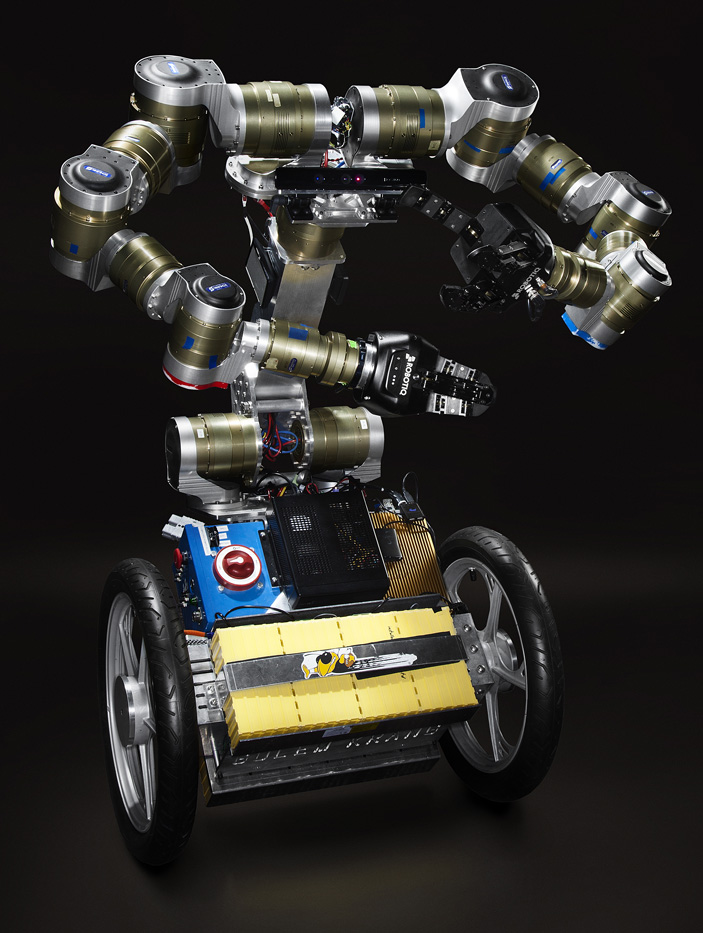
\includegraphics[height=210pt]{fig/KrangPhoto}
  %   \label{fig:krang}
  % }
  % \end{minipage}
  % \begin{minipage}{.38\linewidth}
  %   \centering
  % \subfigure[Chess Grammar]{
  %   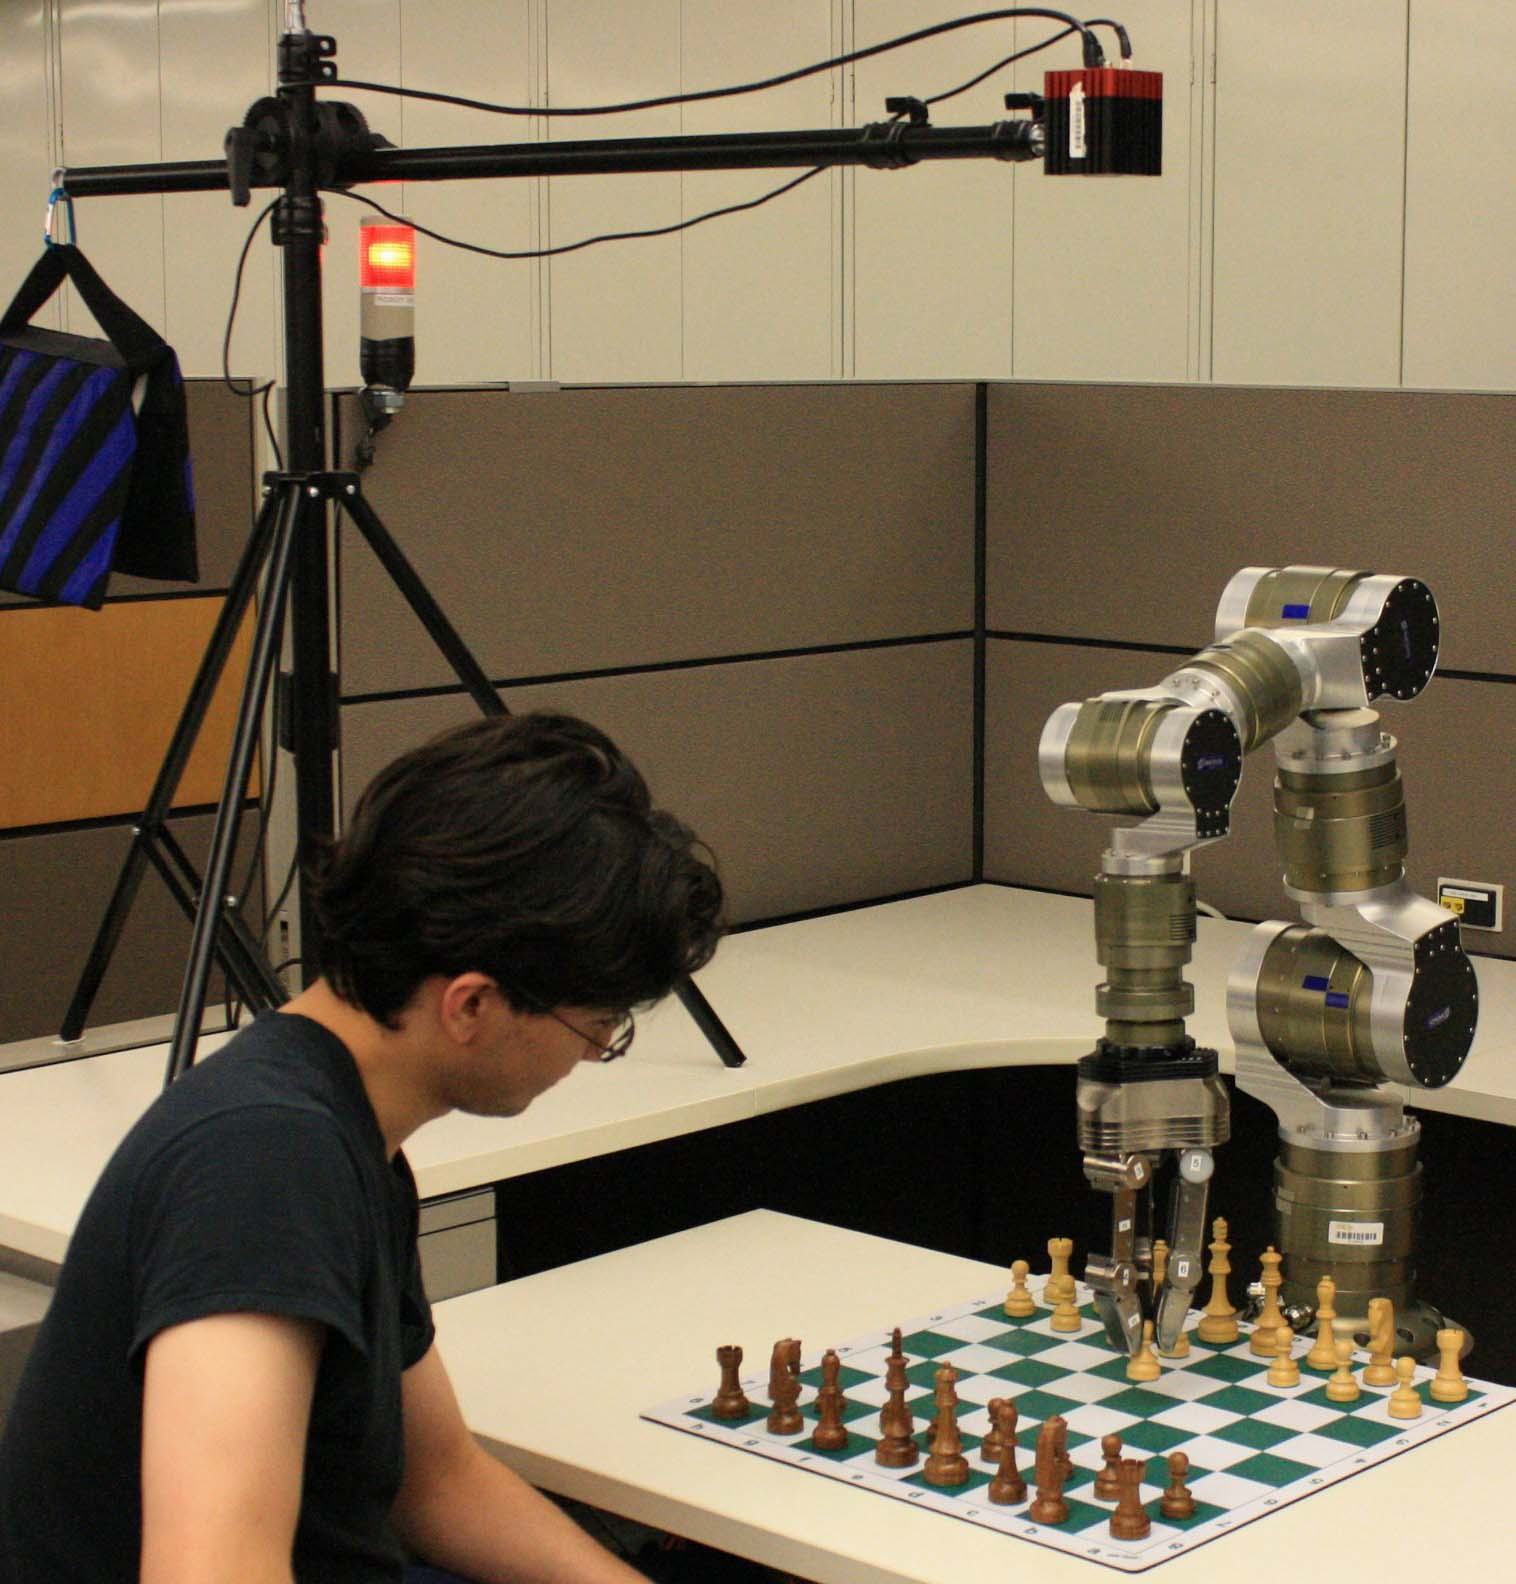
\includegraphics[width=75pt]{fig/chess_setup}
  % }\hspace{-8pt}
  % \subfigure[Yama Grammar]{
  %   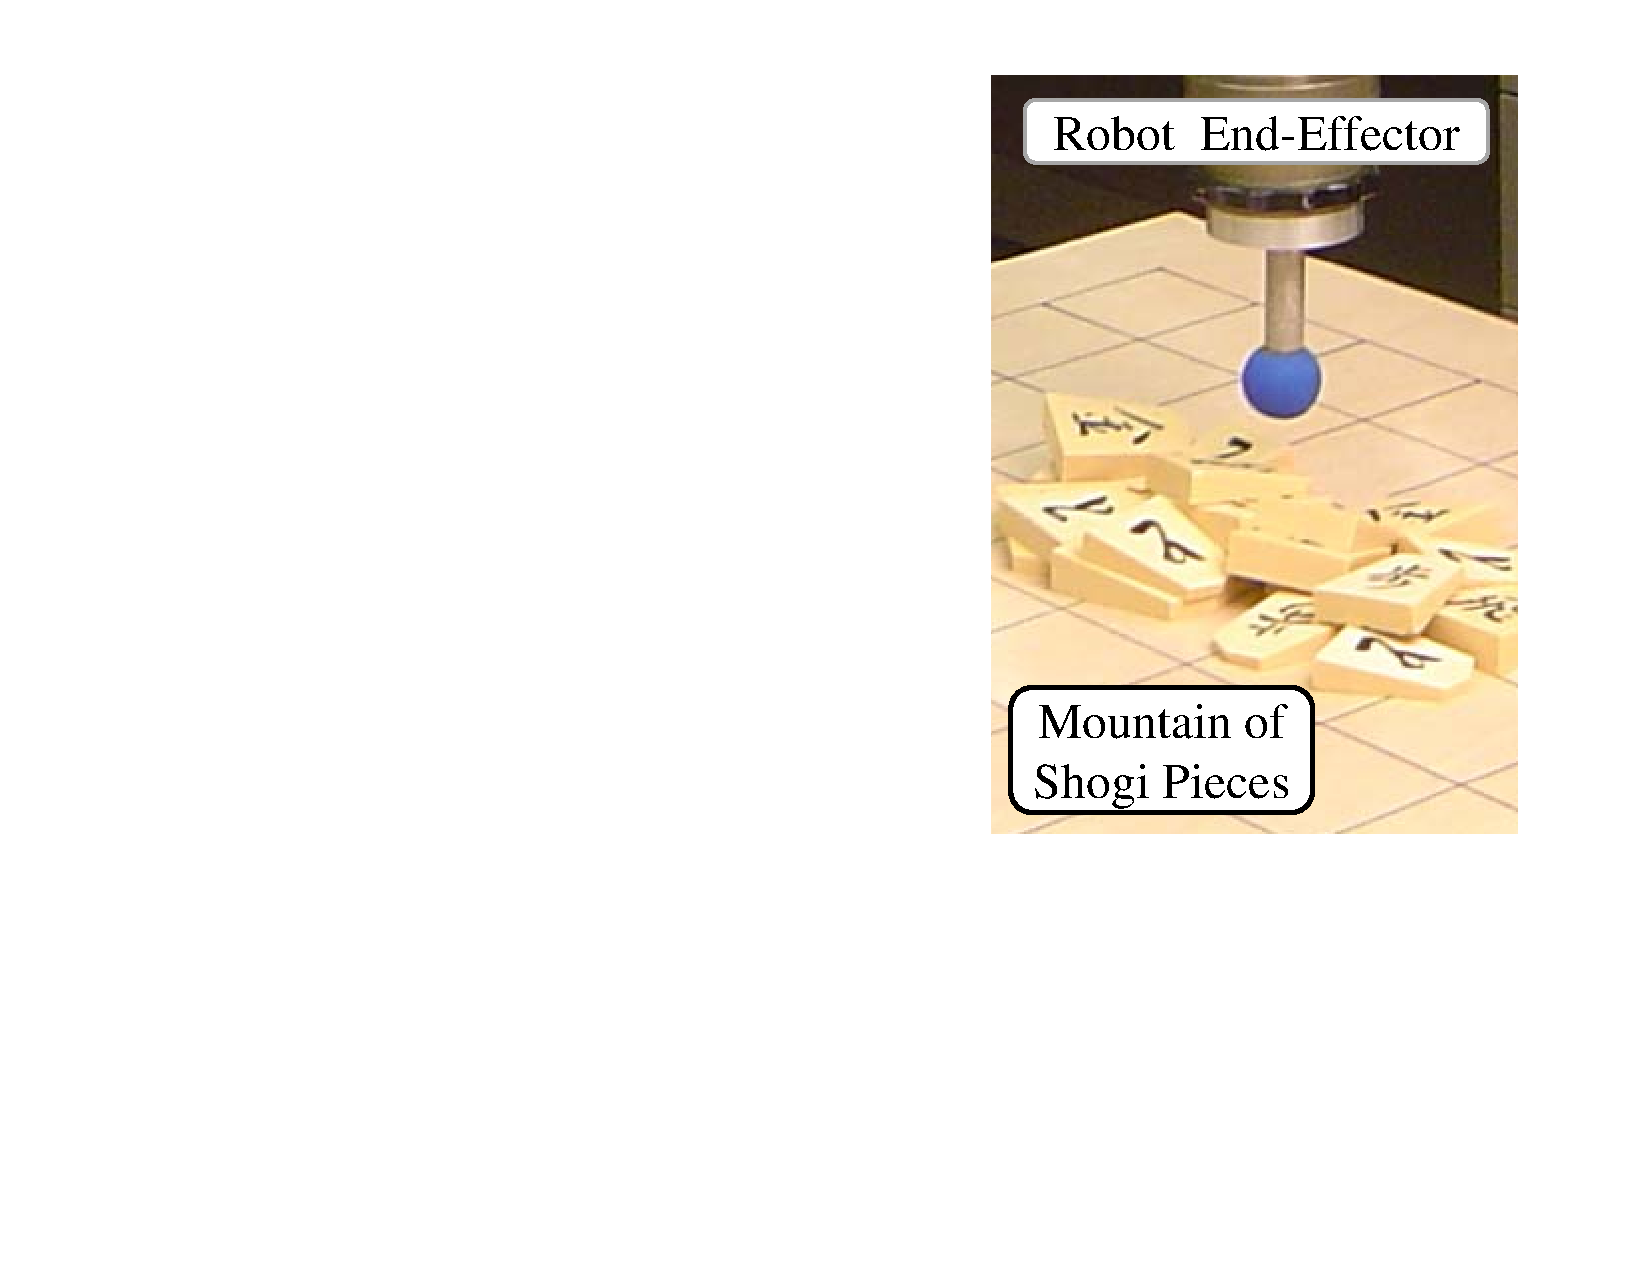
\includegraphics[width=75pt]{fig/yama4}
  % }
  % \end{minipage}
    \caption{HUBO, Golem Krang, and NAO: Robotic Systems where Ach
      provides communications between hardware drivers, perception,
      planning, and control algorithms.}
    \label{fig:app}
\end{figure}


POSIX provides a rich variety of IPC that is well suited for general
purpose information processing, but none are ideal for real-time robot
control.  Typically, a physical process such as a robot is viewed as a
set of continuous, time-varying \emph{signals}.  To control this
physical process with a digital computer, one must \emph{sample} the
signal at discrete time intervals and perform control calculations
using the sampled value. To achieve high-performance control of a
physical system, we must process the latest sample with minimum
latency.  This differs from the requirements of general computing
systems which focus on throughput over latency and favor prior data
over latter data.  Thus, for robot control, it is better to favor new
data over old data whereas nearly all POSIX IPC favors the old
data. This problem is typically referred to as \emph{Head of Line
  (HOL) Blocking}.  The exception to this is POSIX shared
memory. However, synchronization of shared memory is a difficult
programming problem, making the typical and direct use of POSIX shared
memory unfavorable for developing robust systems.  Furthermore, some
parts of the system, such as logging, may need to access older
samples, so this also should be permitted at least on a best-effort
basis.  Since no existing standardized and open source implementation
satisfied our requirements for low-latency exchange of most-recent
samples, we have developed a new open source IPC library.


% POSIX provides a rich variety of IPC mechanisms, but none of them
% fully meet our requirements.  An overview of these mechanisms is given
% in \cite{apue}.  The fundamental difference is that as soon as a new
% sample of the signal is produced, nearly everything no longer cares
% about older samples.  Thus, we want to always favor new data over old
% data whereas nearly all POSIX IPC favors the old data. This problem is
% typically referred to as \emph{Head of Line (HOL) Blocking}.  The
% exception to this is POSIX shared memory. However, synchronization of
% shared memory is a difficult programming problem, making the typical
% and direct use of POSIX shared memory unfavorable for developing
% robust systems.  Furthermore, some parts of the system, such as
% logging, may need to access older samples, so this also should be
% permitted at least on a best-effort basis.  Since no existing
% standardized and open source implementation satisfied our requirements
% for low-latency exchange of most-recent samples, we have developed a
% new open source IPC library.


%% Contributions:
This article discusses a POSIX Interprocess Communication library for
the real-time control of physical processes such as robots, and covers
its application on three humanoid platforms: Golem Krang, HUBO, and
NAO.  This library, called \emph{Ach}, provides a message-bus or
publish-subscribe communication semantics -- similar to other
real-time middleware and robotics programming systems
\cite{dds2007,Quigley09} -- but with the distinguishing feature of
favoring newer data over old.  Ach provides certain advantages making
it suitable for real-time control of physical robotic systems.  In
particular, Ach is formally verified, it is efficient, and it always
provides processes with the most recent data sample.  To our
knowledge, these benefits are unique among existing communications
software.

% Ach has been used to implement communication for several robotic
% systems, shown in \figref{fig:app} and the video attachment to this
% paper \cite{dantam2011chess,dantam2011yama,stilman2010golem}.  The
% performance of these systems verify that the context-switch overhead
% of a multi-process real-time application is acceptable for robot
% control, including manipulation and dynamic balancing.  Our experience
% in developing these systems confirms the benefits in robustness and
% flexibility from a multi-process application.

% This paper is organized as follows: \sectref{sect:reviewipc} reviews
% the various types of POSIX IPC and explains why they do not meet our
% needs.  \sectref{sect:ach} explains the Ach algorithm and
% implementation. \sectref{sect:vb} covers the formal verification of
% Ach and shows quantitative benchmarks. \sectref{sect:discuss}
% discusses the numerous advantages and a few faults of ach.  Finally
% \sectref{sect:conclusion} summarizes the paper and describes some
% possible future directions.

\section{Review of POSIX IPC}

\label{sect:reviewipc}

POSIX provides three main types of general IPC: streams, datagrams,
and shared memory.  We review each of these types and consider why
these general-purpose IPC mechanisms are not ideal for real-time robot
control.  A thorough survey of POSIX IPC is provided in \cite{apue}.

\subsection{Streams}

Stream IPC includes pipes, fifos, local-domain stream sockets, and TCP
sockets.  These IPC mechanisms all expose the \emph{file} abstraction:
a sequence of bytes accessed with {\tt read} and {\tt write}.  All
stream-based IPC suffers from the HOL blocking problem; we must read
all the old bytes before we see any new bytes.  Furthermore, to
prevent blocking of the reading or writing process, we must resort to
more complicated Nonblocking or Asynchronous IO approaches.

\subsection{Datagrams}

\subsubsection{Datagram Sockets}
Datagram sockets perform somewhat better than streams in that they are
less likely to block the sender.  However, they give a variation on
the HOL blocking problem where newer messages are simply lost if a
buffer fills up.  This is unacceptable since we require access to the
most recent data.

\subsubsection{POSIX Message Queues}
While similar to Datagram sockets, POSIX Message Queues include the
feature of message priorities.  The downside is that it is possible to
block if the queue fills up. Consider a process that gets stuck and
stops processing its message queue.  When it starts again, the process
must still read/flush old messages before getting the most recent
sample.

\subsection{Shared Memory}

POSIX shared memory is very fast and one could, by simply overwriting
a variable, always have the latest data.  However, this provides no
recourse for recovering older data that may have been missed.  In
addition, shared memory presents synchronization issues which are
notoriously difficult to solve, making direct shared memory use less
suitable for safety critical real-time control.

The data structure which Ach most closely resembles is the circular
array.  Circular arrays or ring buffers are common data stuctures in
device drivers and real-time programs, and the implimentation in Ach
provides unique features to satisfy our requirements for a
multi-process real-time system.  Typical circular buffers allow only
one producer and one consumer with the view that the producer inserts
data and the consumer removes it.  Our robots have multiple producers
and multiple consumers writing and reading a single sequence of
messages.  A message reader cannot \emph{remove} a message, because
some other process may still need to read it.  Because of this
different design requirement, Ach uses a different data structure and
algorithm in order to perform real-time IPC among multiple processes.

% The Bip Buffer
% \cite{cooke2003bip} is an efficient circular buffer that minimizes
% copying, but it is still designed around a single producer and
% consumer.  The MCRingBuffer \cite{lee2009lock} is a cache-efficient
% design, but it again focuses on the single producer and consumer
% model.

\subsection{Further Considerations}

\subsubsection{Nonblocking and Asynchronous IO approaches} There are
several approaches that allow a single process or thread to perform IO
operations across several file descriptions.  Asynchronous IO (AIO)
may seem to be the most appropriate for this application. However, the
current implementation under Linux is not as mature used as other IPC
mechanisms.  Methods using select/poll/epoll/kqueue are widely used
for network servers. Yet, both AIO and select-based methods only
mitigate the HOL problem, not eliminate it.  Specifically, the sender
will not block, but the receiver must read/flush the old data from the
stream before it can see the most recent sample.

\subsubsection{Priorities}
To our knowledge, none of the stream or datagram forms of IPC consider
the issue of process priorities. Priorities are critical for real-time systems.
When there are two readers that want the next sample, we want the
real-time process, such as a motor driver, to get the data and process
it before a non real-time process, such as a logger, does anything.

\subsection{General, Real-Time and, Robotics Middleware}

In addition to the core POSIX IPC mechanisms, there exist various
messaging middlewares and robot software architectures. However, these
are either not Open Source or not suitable for our multi-process
real-time domain.

The Message Passing Interface (MPI) \cite{gropp1999using} is
ubiquitous in high-performance computing, but its focus is on
maximizing message throughput for networked clusters.  The robot
control domain centers around minimizing sample latency on a single
host.  The Advanced Message Queuing Protocol (AMPQ)
\cite{vinoski2006advanced} is a network message distribution
middleware focused on business applications; it does not address
low-latency real-time systems.  ZeroMQ \cite{zeromq} provides IPC
based on TCP and local-domain sockets which have the HOL blocking
condition.  Remote Procedure Call (RPC) methods such as ONC RPC
\cite{oncrpc} and CORBA \cite{corba} allow synchronous point-to-point
communication but they do not directly allow efficient communication
between multiple senders and receivers and also do not address HOL
blocking.  In contrast, Data Distribution Service \cite{dds2007} is a
publish-subscribe network protocol which may be complementary to the
efficient and formally verified IPC we present here.

The Orocos Real-Time Toolkit \cite{bruyninckx2003real} and NAOqi
\cite{agüero2010behavior} (\autoref{sec:nao_walking}) are two
architectures for robot control, but they do not meet our requirements
for flexible IPC.  iRobot's Aware2.0 is not open source, and Microsoft
Robotics Studio is not open source and does not run on POSIX systems.
ROS \cite{Quigley09} provides open source TCP and UDP message
transports, which suffer from the aforementioned HOL blocking problem.
In conclusion, none of these middlewares met our needs for an open
source, light-weight, and non-HOL blocking IPC.

% The RT-Middleware \cite{ando2005rt}
% framework is based on CORBA, which does not provide a suitably
% lightweight IPC mechanism.

\section{The Ach IPC Library}

\label{sect:ach}

Ach provides a message bus or publish-subscribe style of communication
between multiple writers and multiple readers.  A real-time system has
multiple Ach channels across which individual data samples are
published.  The messages sent on a channel are simple byte arrays, so
arbitrary data may be transmitted such as floating point vectors,
text, images, and binary control messages.  Each channel is
implemented as two circular buffers, (1) a data buffer with variable
sized entries and (2) an index buffer with fixed-size elements
indicating the offsets into the data buffer. These two circular
buffers are written in a channel-specific POSIX shared memory
file. Using this formulation, we solve and formally verify the
synchronization problem exactly once and contain it entirely within
the Ach library.

The Ach interface consists of the following procedures:

\begin{itemize}
  \item {\tt ach\_create}: Create the shared memory region and
    initialize its data structures
  \item {\tt ach\_open}: Open the shared memory file and initialize
    process local channel counters
  \item {\tt ach\_put}: Insert a new message into the channel
  \item {\tt ach\_get}: Receive a message from the channel
  \item {\tt ach\_close}: Close the shared memory file
\end{itemize}

\noindent Channels must be created before they can be opened. Creation
may be done directly by either the reading or writing process, or it
may be done via the shell command, {\tt ach -C channel\_name}, before
the reader or writer start.  This is analogous to the creation of
FIFOs with {\tt mkfifo} called either as a shell command or as a C
function.  After the channel is created, each reader or writer must
open the channel before it can get or put messages.

%and is another example of Ach's flexibility

\begin{figure}[t]
\centering
% \begin{tikzpicture}[->, >=stealth,font=\small]
%   \tikzstyle{cell} = [rectangle,draw=black,minimum width=40,minimum
%   height = 15,node distance=15]
%   \tikzstyle{register} = [rectangle,draw=black,rounded corners];
%   \node[register,name=idxhead] {index\_head};
%   \node[register,name=idxfree, below of=idxhead] {index\_free = 2};


%   \node[cell,name=idx0, right of=idxhead,xshift=40] {$I_0$};
%   \node[cell,name=idx1, below of=idx0] {$I_1$ (free)};
%   \node[cell,name=idx2, below of=idx1] {$I_2$ (free)};
%   \node[cell,name=idx3, below of=idx2] {$I_3$};
%   \node[cell,name=idx4, below of=idx3] {$I_4$};
%   \node[above of=idx0,yshift=-10] {\underline{Index Array}};

%   \node[cell,name=dat0, right of=idx0,xshift=40] {$D_{\rm free}$};
%   \node[cell,name=dat1, below of=dat0] {$D_{18}$};
%   \node[cell,name=dat2, below of=dat1] {$D_{19}$};
%   \node[cell,name=dat3, below of=dat2] {$D_{20}$};
%   \node[cell,name=dat4, below of=dat3] {$D_{\rm free}$};
%   \node[above of=dat0,yshift=-10] {\underline{Data Array}};

%   \node[register,name=dathead,right of=dat2,xshift=40] {data\_head};
%   \node[register,name=datfree,below of=dathead] {data\_free = $n$};
%   \node[register,name=datfree,above of=dathead] {Seq. Num. = 20};


%   \path (idxhead) edge (idx1.west);
%   \path (idx3.east) edge (dat1.west);
%   \path (idx4.east) edge (dat2.west);
%   \path (idx0.east) edge (dat3.west);
%   \path (dathead) edge (dat4.east);
% \end{tikzpicture}

\ovalbox{
  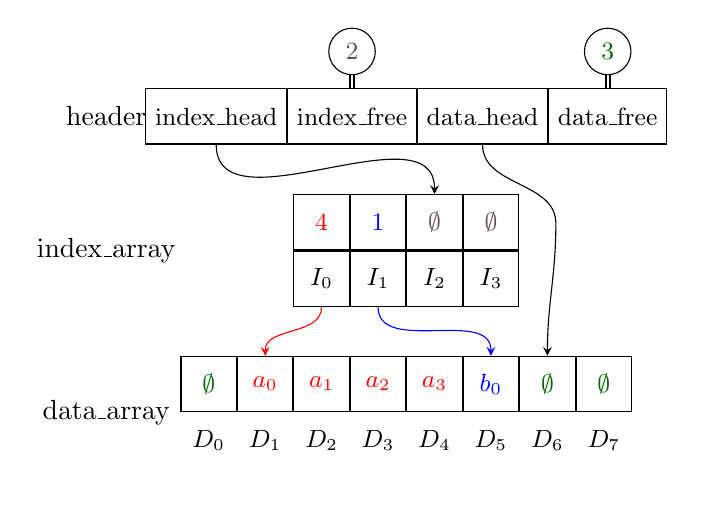
\begin{tikzpicture}
  \tikzstyle{cell} = [rectangle,minimum height=2.0em,minimum
  width=2.00em, font=\small,draw=black]
  \tikzstyle{vcell} = [rectangle,minimum height=2.0em,minimum
  width=2.00em, font=\small,draw=white]

  \tikzstyle{ref} =[->, >=stealth,out=-90,in=90]

  \node [matrix,nodes=draw] (header)
  {
    \node[cell,name=idxhead]{index\_head}; &
    \node[cell,name=idxfree]{index\_free}; &
    \node[cell,name=dathead]{data\_head}; &
    \node[cell,name=datfree]{data\_free};\\
  };
  \node[draw,font=\small,circle,above
  of=idxfree,name=vif,color=pink!40!black,draw=black,yshift=-0.5em] {2};
  \node[draw,font=\small,circle,above
  of=datfree,name=vdf,color=green!40!black,draw=black,yshift=-.5em] {3};

  \node [matrix,below of=header,yshift=-2.0em] (index)
  {
    \node[cell,name=n0,color=red,draw=black]{$4$}; &
    \node[cell,name=n1,color=blue,draw=black]{$1$}; &
    \node[cell,name=n2,color=pink!40!black,draw=black]{$\emptyset$}; &
    \node[cell,name=n3,color=pink!40!black,draw=black]{$\emptyset$}; \\
    \node[cell,name=i0,font=\small]{$I_0$}; &
    \node[cell,name=i1,font=\small]{$I_1$}; &
    \node[cell,name=i2,font=\small]{$I_2$}; &
    \node[cell,name=i3,font=\small]{$I_3$}; \\
  };
  \node [matrix,below of=index,yshift=-3.0em] (data)
  {
    \node[cell,name=v0,color=green!40!black,draw=black]{$\emptyset$}; &
    \node[cell,name=v1,color=red, draw=black]{$a_0$}; &
    \node[cell,name=v2,color=red,draw=black]{$a_1$}; &
    \node[cell,name=v3,color=red,draw=black]{$a_2$}; &
    \node[cell,name=v4,color=red,draw=black]{$a_3$}; &
    \node[cell,name=v5,color=blue,draw=black]{$b_0$}; &
    \node[cell,name=v6,color=green!40!black,draw=black]{$\emptyset$}; &
    \node[cell,name=v7,color=green!40!black,draw=black]{$\emptyset$}; \\
    \node[vcell,name=d0]{$D_0$}; &
    \node[vcell,name=d1]{$D_1$}; &
    \node[vcell,name=d2]{$D_2$}; &
    \node[vcell,name=d3]{$D_3$}; &
    \node[vcell,name=d4]{$D_4$}; &
    \node[vcell,name=d5]{$D_5$}; &
    \node[vcell,name=d6]{$D_6$}; &
    \node[vcell,name=d7]{$D_7$}; \\
  };
  \node[name=hlabel,left of=header,xshift=-8em] {header};
  \node[name=ilabel,left of=index,xshift=-8em] {index\_array};
  \node[name=dlabel,left of=data,xshift=-8em] {data\_array};
  %\path (hlabel) edge[dotted] (idxhead);
  %\path (ilabel) edge[dotted] (i0);
  %\path (dlabel) edge[dotted] (d0);

  \path (idxhead.south) edge[ref,out=-90,in=90] (n2.north);
  \node[coordinate,name=d0dot,right of=i3,xshift=-0.5em,yshift=2em] {};
  \path (dathead) edge[out=-90,in=90] (d0dot);
  \path (d0dot) edge[ref,out=-90,in=90] (v6);

  \path (i1) edge[ref,color=blue] (v5);
  \path (i0) edge[ref,color=red] (v1);

  \path (idxfree) edge[double,thick] (vif);
  \path (datfree) edge[double,thick] (vdf);

\end{tikzpicture}
}
\caption{Logical Memory Structure for an Ach shared memory file. In
  this example, $I_0$ points to a four byte message starting at $D_1$,
  and $I_1$ points to a one byte message starting at $D_5$.  The next
  inserted message will use index cell $I_2$ and start at $D_6$.
  There are two free index cells and three free data bytes.  Both
  arrays are circular and wrap around when the end is reached.}
\label{fig:chanstruct}
\vspace{-15pt}
\end{figure}

\subsection{Channel Data Structure}

The core data structure of an Ach channel is a pair of circular arrays
located in the POSIX shared memory file, \autoref{fig:chanstruct}.  The
data array contains variable sized elements which store the actual
message frames sent through the Ach channel.  The index array contains
fixed size elements where each element contains both an offset into
the data array and the length of that element.  A head offset into
each array indicates both the place to insert the next data and the
location of the most recent message frame.  This pair of circular
arrays allows readers to find the variable sized message frames by
first looking at a known offset in the fixed-sized index array.

Access to the channel is synchronized using a mutex and condition
variable.  This allows readers to either periodically poll the channel
for new data or to wait on the condition variable until a writer has
posted a new message.  Using a read/write lock instead would have
allowed only polling.  Additionally, synchronization using a mutex
prevents starvation and enables proper priority inheritance between
processes, important to maintaining real-time performance.

% Diagram of Shared Memory area


\subsection{Core Procedures}
Two procedures compose the core of ach: {\tt ach\_put} and {\tt ach\_get} which we describe in pseudocode.
\vspace{+5pt}
\noindent \subsubsection{ach\_put}
The procedure {\tt ach\_put} inserts new messages into the channel.
Its function is analogous to {\tt write}, {\tt sendmsg}, and {\tt
  mq\_send}.  The procedure is given a pointer to the shared memory
region for the channel and a byte array containing the message to
post.  There are four broad steps to the procedure:

{\small
\begin{enumerate}[(1)]
  %\setcounter{enumi}{-1}
\item Get an index entry.  If there is at least one free index entry,
  use it.  Otherwise, clear the oldest index entry and its
  corresponding message in the data array.
\item Make room in the data array.  If there is enough room already,
  continue.  Otherwise, repeatedly free the oldest message until there
  is enough room.
\item Copy the message into data array.
\item Update the offset and free counts in the channel structure.
\end{enumerate}}

% \begin{procedure}[t!]
%   \small
%   \KwIn{c : ach channel \tcp*{shared memory file}}
%   \KwIn{b : byte array \tcp*{message buffer}}
%   \KwIn{n : integer \tcp*{length of message}}
%   \KwOut{ status : integer \tcp*{status code}}
%   \lIf{ n $>$ {length}(c.data\_array) }{
%     \Return{OVERFLOW}\;}
%   \textsc{lock}($c$); \tcp{take the mutex}
%   \tcc{Get a index entry}
%   \nllabel{alg:put:idxstart}
%   \If{ 0 = c.index\_free } {
%     $c.data\_free\,+\!\!= c.index\_array[c.index\_head].size$\;
%     $c.index\_free \leftarrow 1$\;
%     \nllabel{alg:put:idxend}
%   }
%   \tcc{Make room in data array}
%   $i \leftarrow (c.index\_head + c.index\_free)\ \%\ c.index\_cnt$\;
%   \nllabel{alg:put:datstart}
%   \While{ c.data\_free $<$ n } {
%     $c.data\_free\,+\!\!= c.index\_array[i].size$\;
%     $c.index\_free+\!\!+$\;
%     $i \leftarrow (i + 1)\ \%\ c.index\_cnt$\;
%     \nllabel{alg:put:datend}
%   }
%   \tcc{Copy Buffer}
%   \eIf{c.data\_size - c.data\_head $\geq$ n} {
%     \nllabel{alg:put:cpystart}
%     \tcc{Simple Copy}
%     \textsc{memcpy}($c.data\_array + c.data\_head$, $b$, $n$)\;
%   }{
%     \tcc{Wraparound Copy}
%     $e \leftarrow c.data\_size - c.data\_head$\;
%     \textsc{memcpy}($c.data\_array + c.data\_head$, $b$, $e$)\;
%     \textsc{memcpy}($c.data\_array$, $b + e$, $n - e$)\;
%     \nllabel{alg:put:cpyend}
%   }

%   \tcc{Modify Counts}

%   \nllabel{alg:put:cntstart}
%   $c.index\_array[c.index\_head].size = n$\;
%   $c.index\_array[c.index\_head].offset = c.data\_head$\;
%   $c.data\_head \leftarrow (c.data\_head + n)\ \%\ length(c.data\_array)$\;
%   $c.data\_free\,-\!\!= n$\;
%   $c.index\_head \leftarrow (c.index\_head + 1)\ \%\ c.index\_cnt$\;
%   $c.index\_free -\!\!-$\;
%   \nllabel{alg:put:cntend}

%   \textsc{unlock}($c$); \tcp{release the mutex}
%   \textsc{notify}($c$); \tcp{wake readers on cond. var.}

%   \Return{OK}\;
%   % \caption{ach\_put(c,b,n)}
%   \caption{ach-put()}
%   \label{alg:achput}
% \end{procedure}

% \begin{procedure}[t!]
%   \small
%   \KwIn{$c$ : ach channel \tcp*{shared memory file}}
%   \KwIn{$b$ : byte array \tcp*{storage for message}}
%   \KwIn{$n$ : integer \tcp*{size of b}}
%   \KwIn{$s$ : integer \tcp*{last seq. num. seen}}
%   \KwIn{$i$ : integer \tcp*{next index to read}}
%   \KwIn{$o_w$ : boolean \tcp*{wait for new message?}}
%   \KwIn{$o_l$ : boolean \tcp*{get newest msg.?}}
%   \KwOut{integer $\times$ integer \tcp*{size,
%       status}}
%   \KwOut{$s$ : integer \tcp*{new last seq. num.}}
%   \KwOut{$i$ : integer \tcp*{new next index}}
%   \textsc{lock}($c$); \tcp{take the mutex}
%   \If{ $c.seq\_num = s \land o_w$}{
%     \textsc{wait}($c$); \tcp{condition variable wait}
%   }

%   \If{$c.last\_seq = s \lor 0 = c.last\_seq$} {
%     \textsc{unlock}(c)\;
%     \Return{$(0 \times STALE)$}; \tcp{no entries}
%   }
%   \tcc{Find index array offset, j}
%   \If{ $o_l$ } {
%     \tcc{newest index}
%     $j \leftarrow
%     (c.index\_head + c.index\_cnt -1)\ \%\ c.index\_cnt$\;
%   }\ElseIf{$\neg o_l \land c.index\_array[i].seq\_num = s + 1$} {
%     $j \leftarrow i$; \tcp{next index}
%   }\Else {
%     \tcc{oldest index}
%     $j \leftarrow (c.index\_head + c.index\_free)\ \%\ c.index\_cnt$\;
%   }
%   \tcc{Now read frame from data array}
%   $x = c.index\_array[j]$\;
%   \If{$x.size > n$} {
%     \textsc{unlock}(c)\;
%     \Return{$(x.size \times OVERFLOW)$};
%   }
%   \eIf{$x.offset + x.size < c.data\_size$}{
%     \textsc{memcpy}($b$, $c.data\_array + x.offset$, $x.size$)\;
%   }{
%     $e = c.data\_size - x.offset$\;
%     \textsc{memcpy}($b$, $c.data\_array + x.offset$, $e$)\;
%     \textsc{memcpy}($b + e$, $c.data\_array$, $x.size - e$)\;
%   }
%   $s' \leftarrow s$\;
%   $s \leftarrow x.seq\_num$\;
%   \textsc{unlock}(c)\;
%   $i \leftarrow (i + 1)\ \%\ c.index\_cnt$\;
%   \eIf{ $x.seq\_num > s' + 1$ } {
%     \Return{$(x.size \times MISSED)$}\;
%   }{
%     \Return{$(x.size \times OK)$}\;
%   }
%   %\caption{ach\_get($c$,$b$,$n$,$s$,$i$,$o_w$,$o_l$)}
%   \caption{ach-get()}
% \end{procedure}

\noindent\subsubsection{ach\_get}
The procedure {\tt ach\_get} receives a message from the channel.  Its
function is analogous to {\tt read}, {\tt recvmsg}, and {\tt
  mq\_receive}.  The procedure takes a pointer to the shared memory
region, a storage buffer to copy the message to, the last message
sequence number received, the next index offset to check for a
message, and option flags indicating whether to block waiting for a
new message and whether to return the newest message bypassing any
older unseen messages.  There are four broad steps to the procedure:
{\small
\begin{enumerate}[(1)]
  %\setcounter{enumi}{-1}
  \item If we are to wait for a new message and there is no new message,
    then wait.  Otherwise, if there are no new messages,
    return a status code indicating this fact.
  \item Find the index entry to use.  If we are to return the newest
    message, use that entry.  Otherwise, if the next entry we expected
    to use contains the next sequence number we expect to see, use
    that entry.  Otherwise, use the oldest entry.
  \item According to the offset and size from the selected index
    entry, copy the message from the data array into the provided
    storage buffer.
  \item Update the sequence number count and next index entry offset
    for this receiver.
\end{enumerate}}


\section{Case Studies}

\subsection{Dynamic Balance on Golem Krang}

Golem Krang \cite{stilman2010golem} is a dynamically balancing
bi-manual mobile manipulator designed and built at the Georgia Tech
Humanoid Robotics Lab.  All the real-time control for Krang is
implemented through the Ach IPC library.  This approach has produced
software that is both robust and modular, minimizing system failures
and allowing significant code reuse both within Krang with other
projects \cite{dantam2013tro} sharing the same hardware components.


\begin{figure}
  \subfigure[Golem Krang]{
    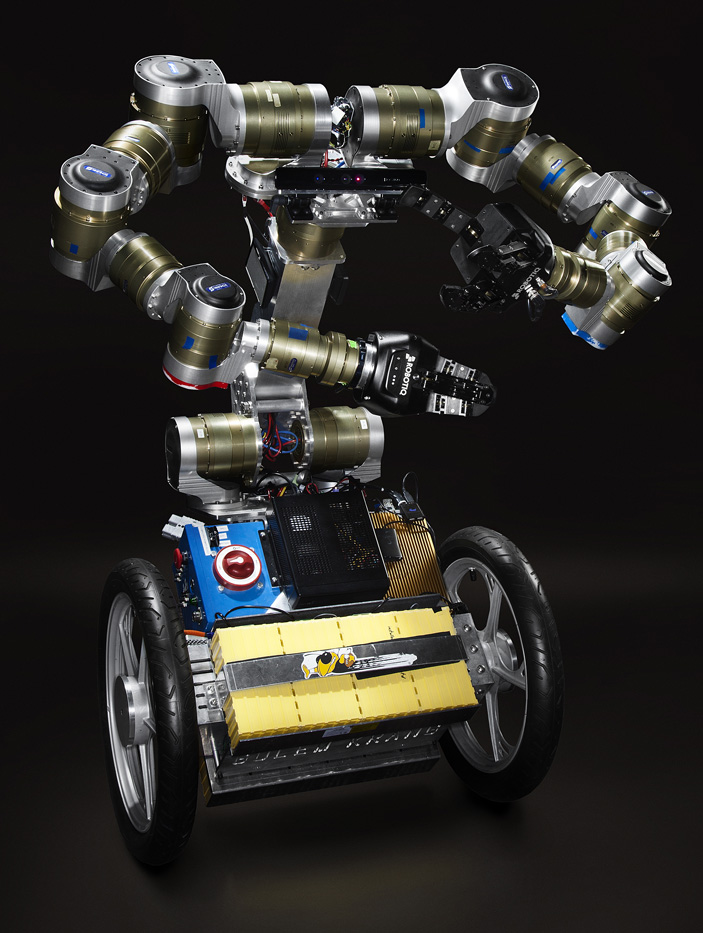
\includegraphics[height=130pt]{./fig/KrangPhoto}
    \label{fig:krang}
  }
  \subfigure[Hubo 2 Plus]{
    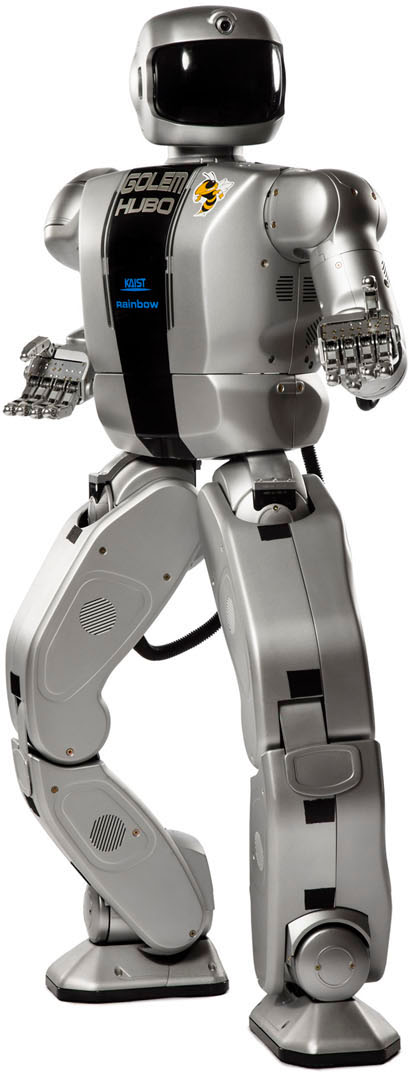
\includegraphics[height=130pt]{./fig/hubo-pose}
    \label{fig:hubo}
  }
  \subfigure[NAO]{
    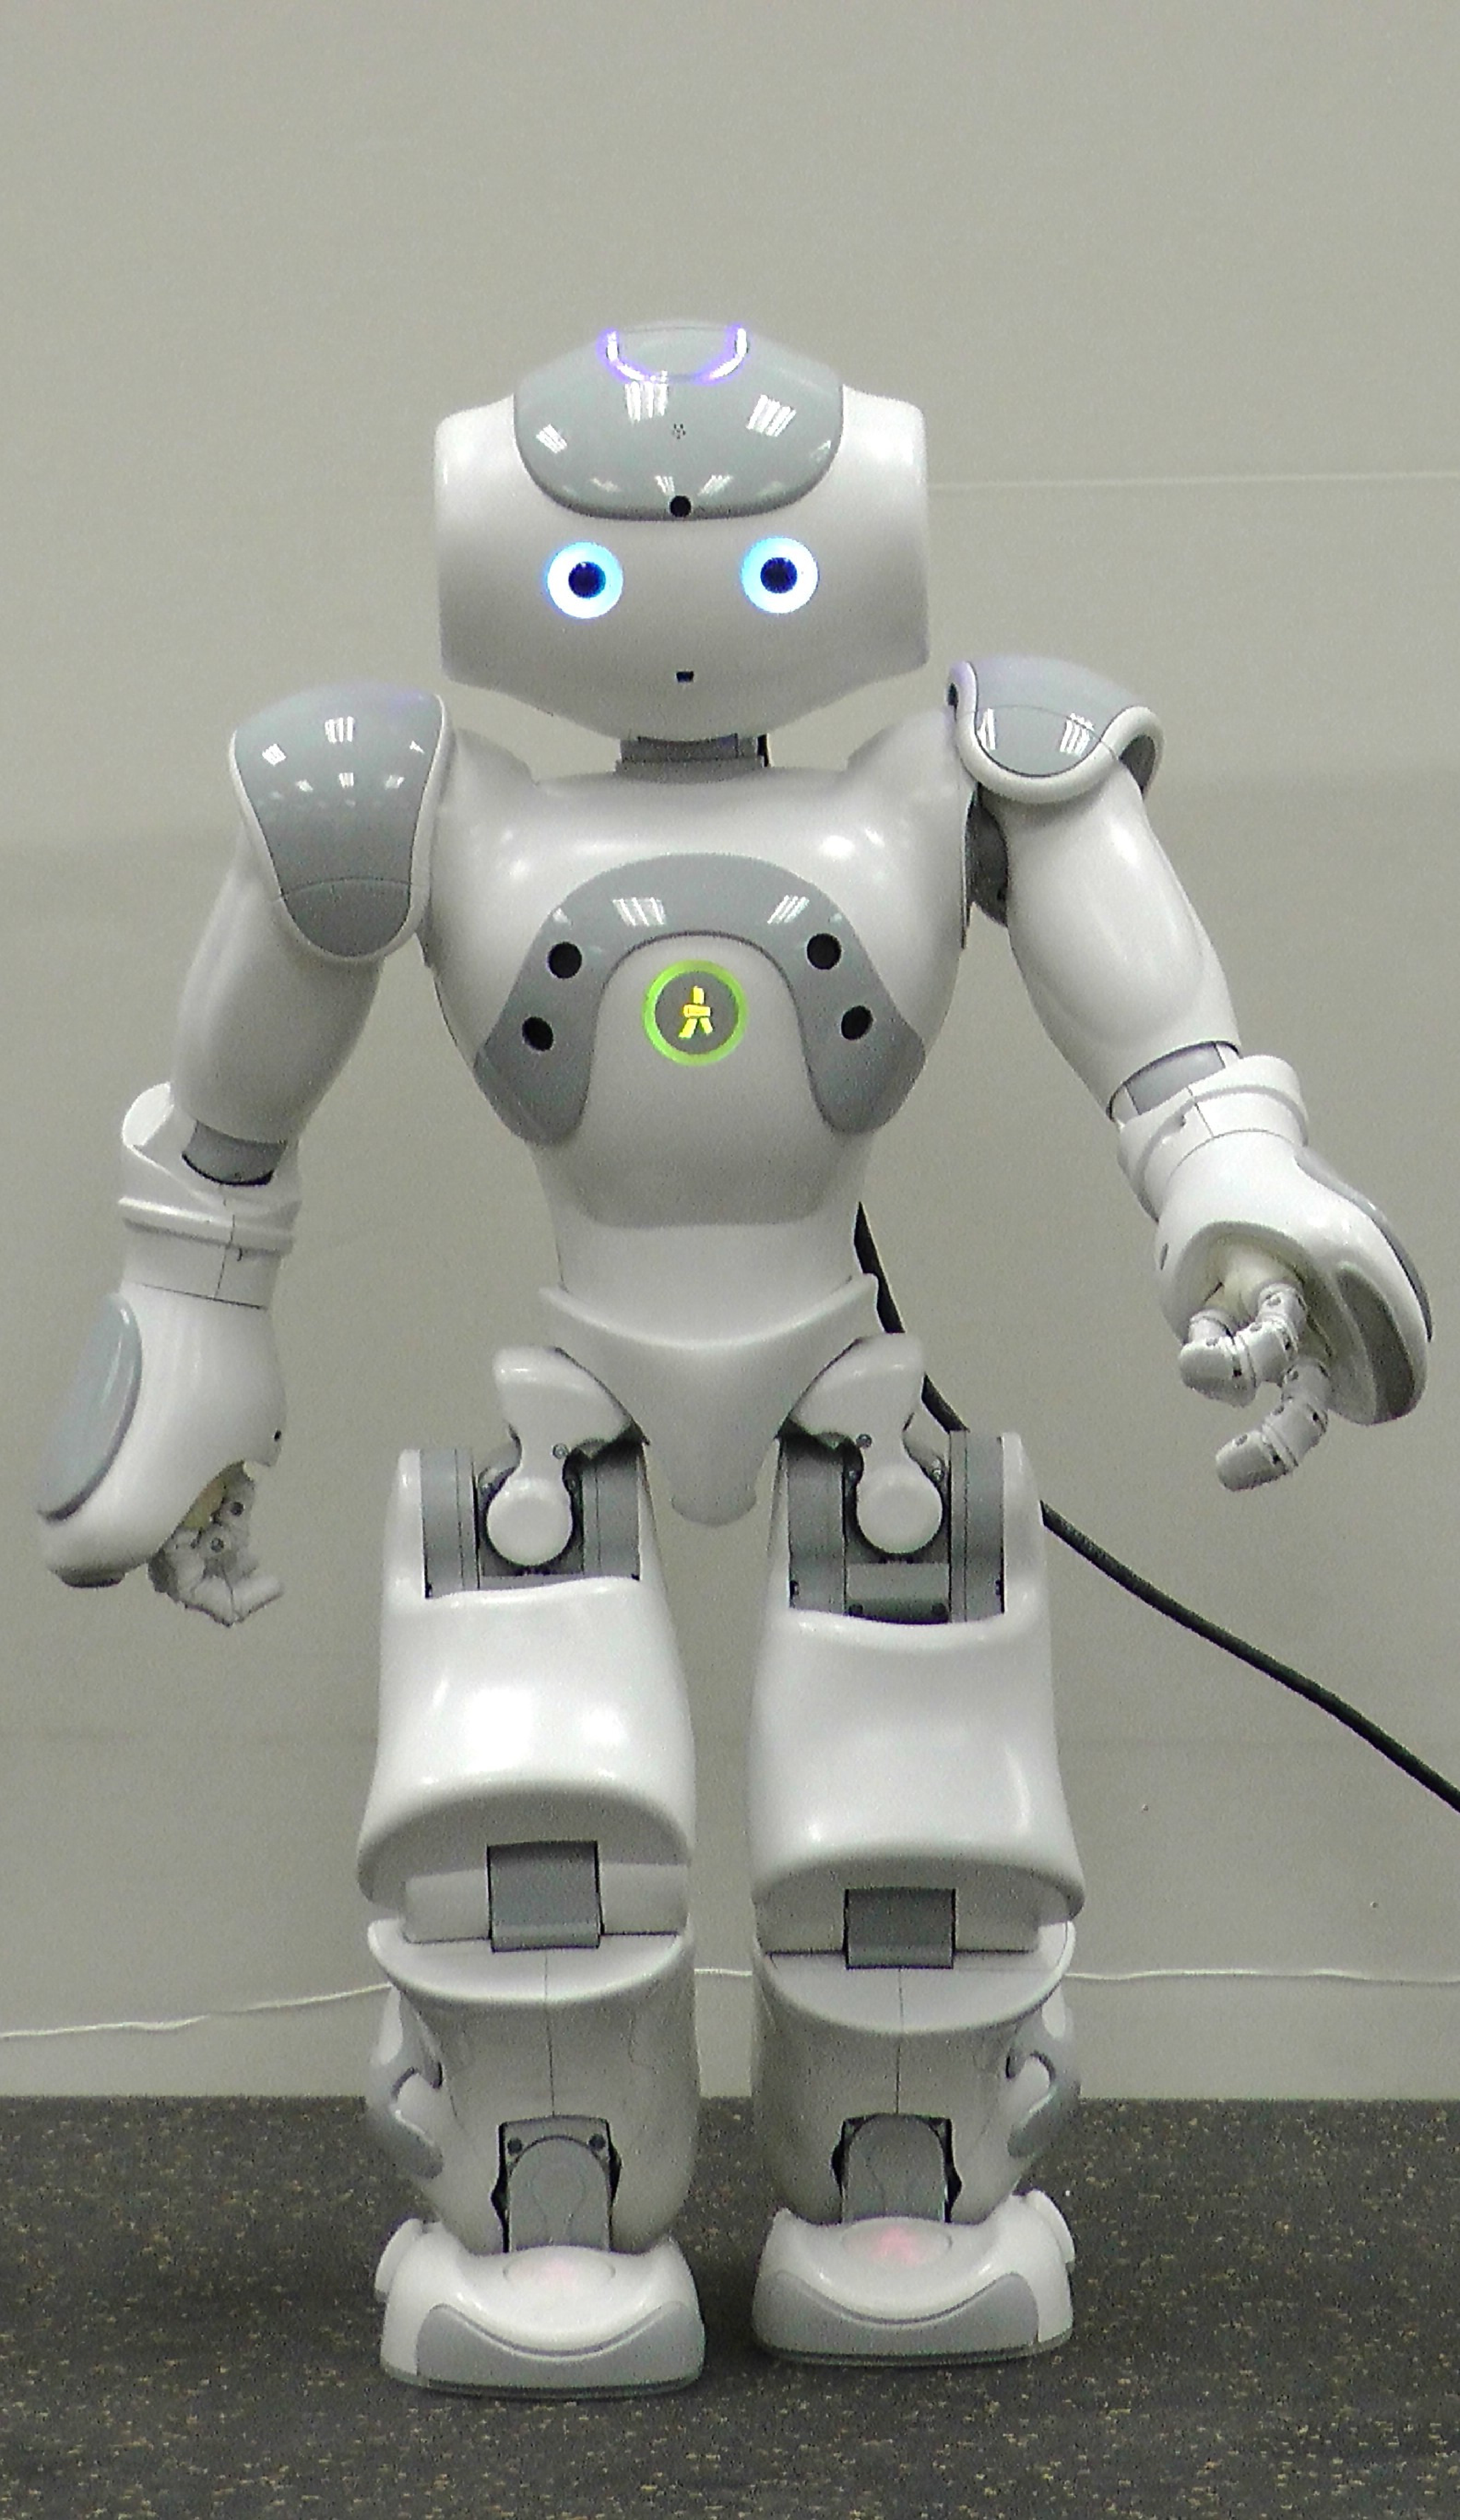
\includegraphics[height=130pt]{./fig/nao_stand}
    \label{fig:nao}
  }
\end{figure}

%\begin{figure}
  %\caption{The HUBO 2 Plus}
  %\label{fig:hubo}
%\end{figure}

\begin{figure}
  %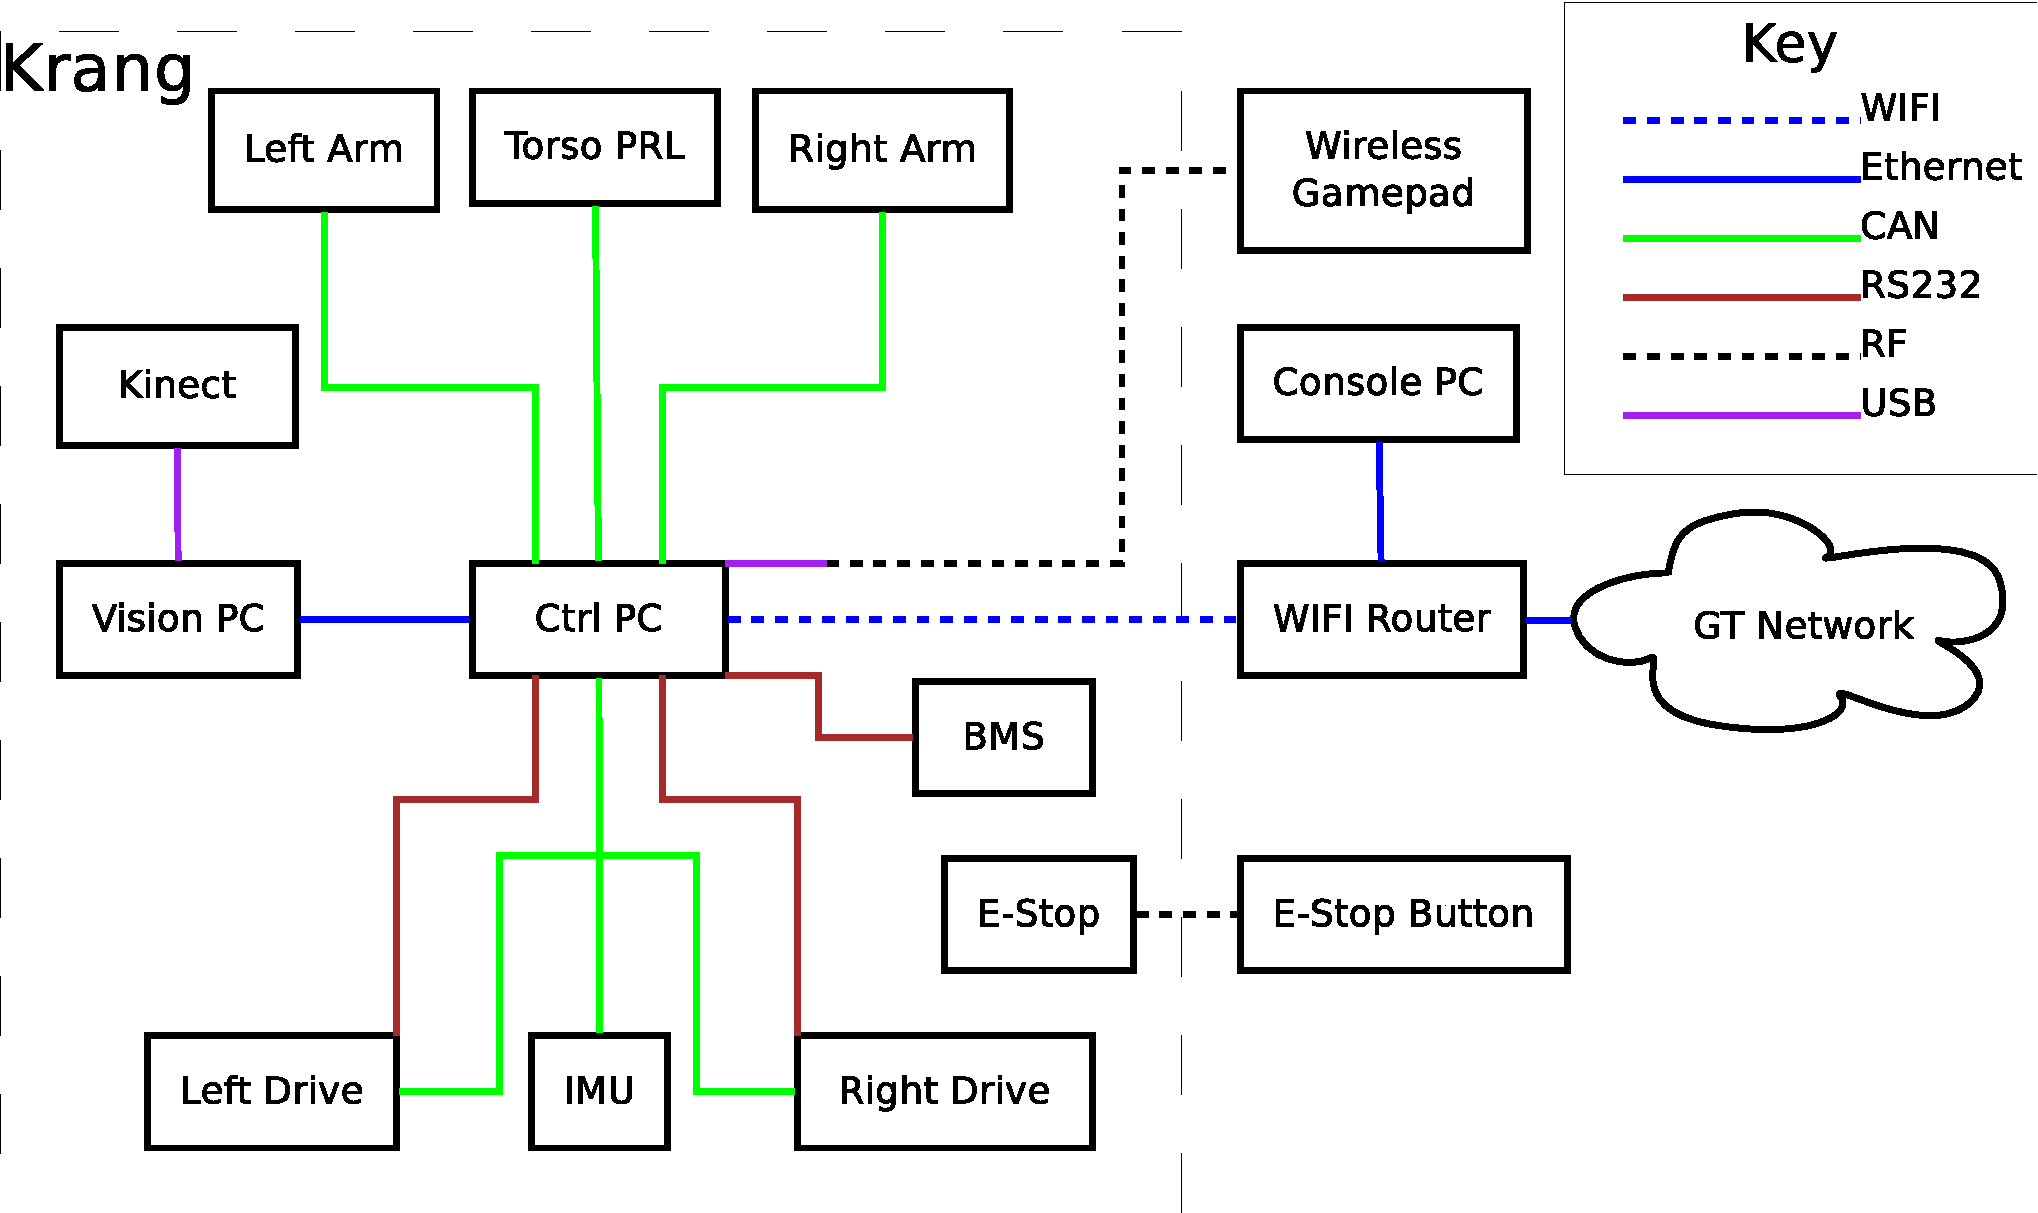
\includegraphics[width=.5\textwidth]{fig/krangblock}
  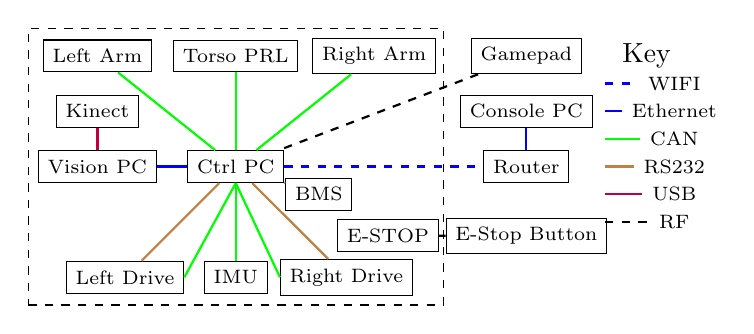
\begin{tikzpicture}
    \tikzstyle{block} = [rectangle,draw=black,font=\scriptsize,node
    distance=3em];
    \tikzstyle{keyitem} = [font=\scriptsize, node distance=1em];
    \tikzstyle{can} = [green,thick];
    \tikzstyle{rs232} = [brown,thick];
    \tikzstyle{wifi} = [blue,dashed,thick];
    \tikzstyle{ethernet} = [blue,thick];
    \tikzstyle{rf} = [black,dashed,thick];
    \tikzstyle{usb} = [purple,thick];

    \node[block,name=krang,minimum width=15em,minimum
    height=10em,dashed] {};
    \node[block,name=ctrlpc] {Ctrl PC};

    \node[block,name=torsoprl,above of=ctrlpc,yshift=1em] {Torso PRL};
    \node[block,name=leftarm,left of=torsoprl,xshift=-2em] {Left Arm};
    \node[block,name=rightarm,right of=torsoprl,xshift=2em] {Right Arm};

    \node[block,name=imu,below of=ctrlpc,yshift=-1em] {IMU};
    \node[block,name=leftdrive,left of=imu,xshift=-1em] {Left Drive};
    \node[block,name=rightdrive,right of=imu,xshift=1em] {Right Drive};

    \node[block,name=visionpc,left of=ctrlpc,xshift=-2em,yshift=-0em] {Vision PC};
    \node[block,name=kinect,above of=visionpc,yshift=-1em] {Kinect};

    \node[block,name=bms,right of=ctrlpc,yshift=-1em] {BMS};
    \node[block,name=estop,right of=bms,yshift=-1.5em,xshift=-.5em] {E-STOP};

    \node[block,name=router,right of=ctrlpc,xshift=7.5em] {Router};
    \node[block,name=consolepc,above of=router,yshift=-1em] {Console PC};
    \node[block,name=gamepad,above of=consolepc,yshift=-1em] {Gamepad};
    \node[block,name=ebutton,below of=router,yshift=.5em] {E-Stop Button};

    \path (ctrlpc.north) edge[can] (torsoprl);
    \path (ctrlpc) edge[can] (leftarm);
    \path (ctrlpc) edge[can] (rightarm);
    \path (ctrlpc.south) edge[can] (imu);
    \path (ctrlpc.south) edge[can] (leftdrive.east);
    \path (ctrlpc.south) edge[can] (rightdrive.west);

    \path(ctrlpc) edge[ethernet] (visionpc);
    \path(visionpc) edge[usb] (kinect);

    \path(ctrlpc) edge[rs232] (leftdrive);
    \path(ctrlpc) edge[rs232] (rightdrive);

    \path(ctrlpc) edge[rs232] (bms);

    \path(gamepad) edge[rf] (ctrlpc);
    \path(consolepc) edge[ethernet] (router);
    \path(ctrlpc) edge[wifi] (router);
    \path(estop) edge[rf] (ebutton);


    \node[right of=gamepad,name=key,xshift=1.5em] {Key};
    \node[keyitem,name=wifi,below of=key,xshift=1em] {WIFI};
    \node[keyitem,name=ethernet,below of=wifi] {Ethernet};
    \node[keyitem,name=can,below of=ethernet] {CAN};
    \node[keyitem,name=rs232,below of=can] {RS232};
    \node[keyitem,name=usb,below of=rs232] {USB};
    \node[keyitem,name=rf,below of=usb] {RF};

    \path ($(key)+(-1.5em,-1em)$) edge[wifi] (wifi);
    \path ($(key)+(-1.5em,-2em)$) edge[ethernet] (ethernet);
    \path ($(key)+(-1.5em,-3em)$) edge[can] (can);
    \path ($(key)+(-1.5em,-4em)$) edge[rs232] (rs232);
    \path ($(key)+(-1.5em,-5em)$) edge[usb] (usb);
    \path ($(key)+(-1.5em,-6em)$) edge[rf] (rf);

  \end{tikzpicture}
  \caption{Block diagram of electronic components on Golem
    Krang. Blocks inside the dashed line are onboard and blocks
    outside are offboard.}
  \label{fig:krangblock}
\end{figure}

The electronic components of Golem Krang are summarized in the block
diagram of \autoref{fig:krangblock}.  The real-time control software
runs on the Pentium-M Control PC under Ubuntu Linux.  Krang also
contains a secondary Intel i7 PC for vision processing, separate from
the real-time control system discussed in this paper.  The Control PC
communicates over eight Controller Area Network buses to embedded
microcontrollers for the wheels, Inertial Measurement Unit (IMU),
torso, and arms.  Each wheel is controlled by an AMC servocontroller.
The torso is actuated using three Schunk PRL motor modules. Each arm
is a Schunk LWA3 with a wrist-mounted ATI force-torque sensor and
Robotiq Adaptive Gripper.  The battery management system (BMS)
monitors voltage of the lithium battery cells.  To achieve dynamic
balance and manipulation, software on the Control PC must gather state
updates from the arms, wheels, and IMU, then compute the inputs for
arms and wheels, all at the desired rate of one kilohertz.


\begin{figure}
  %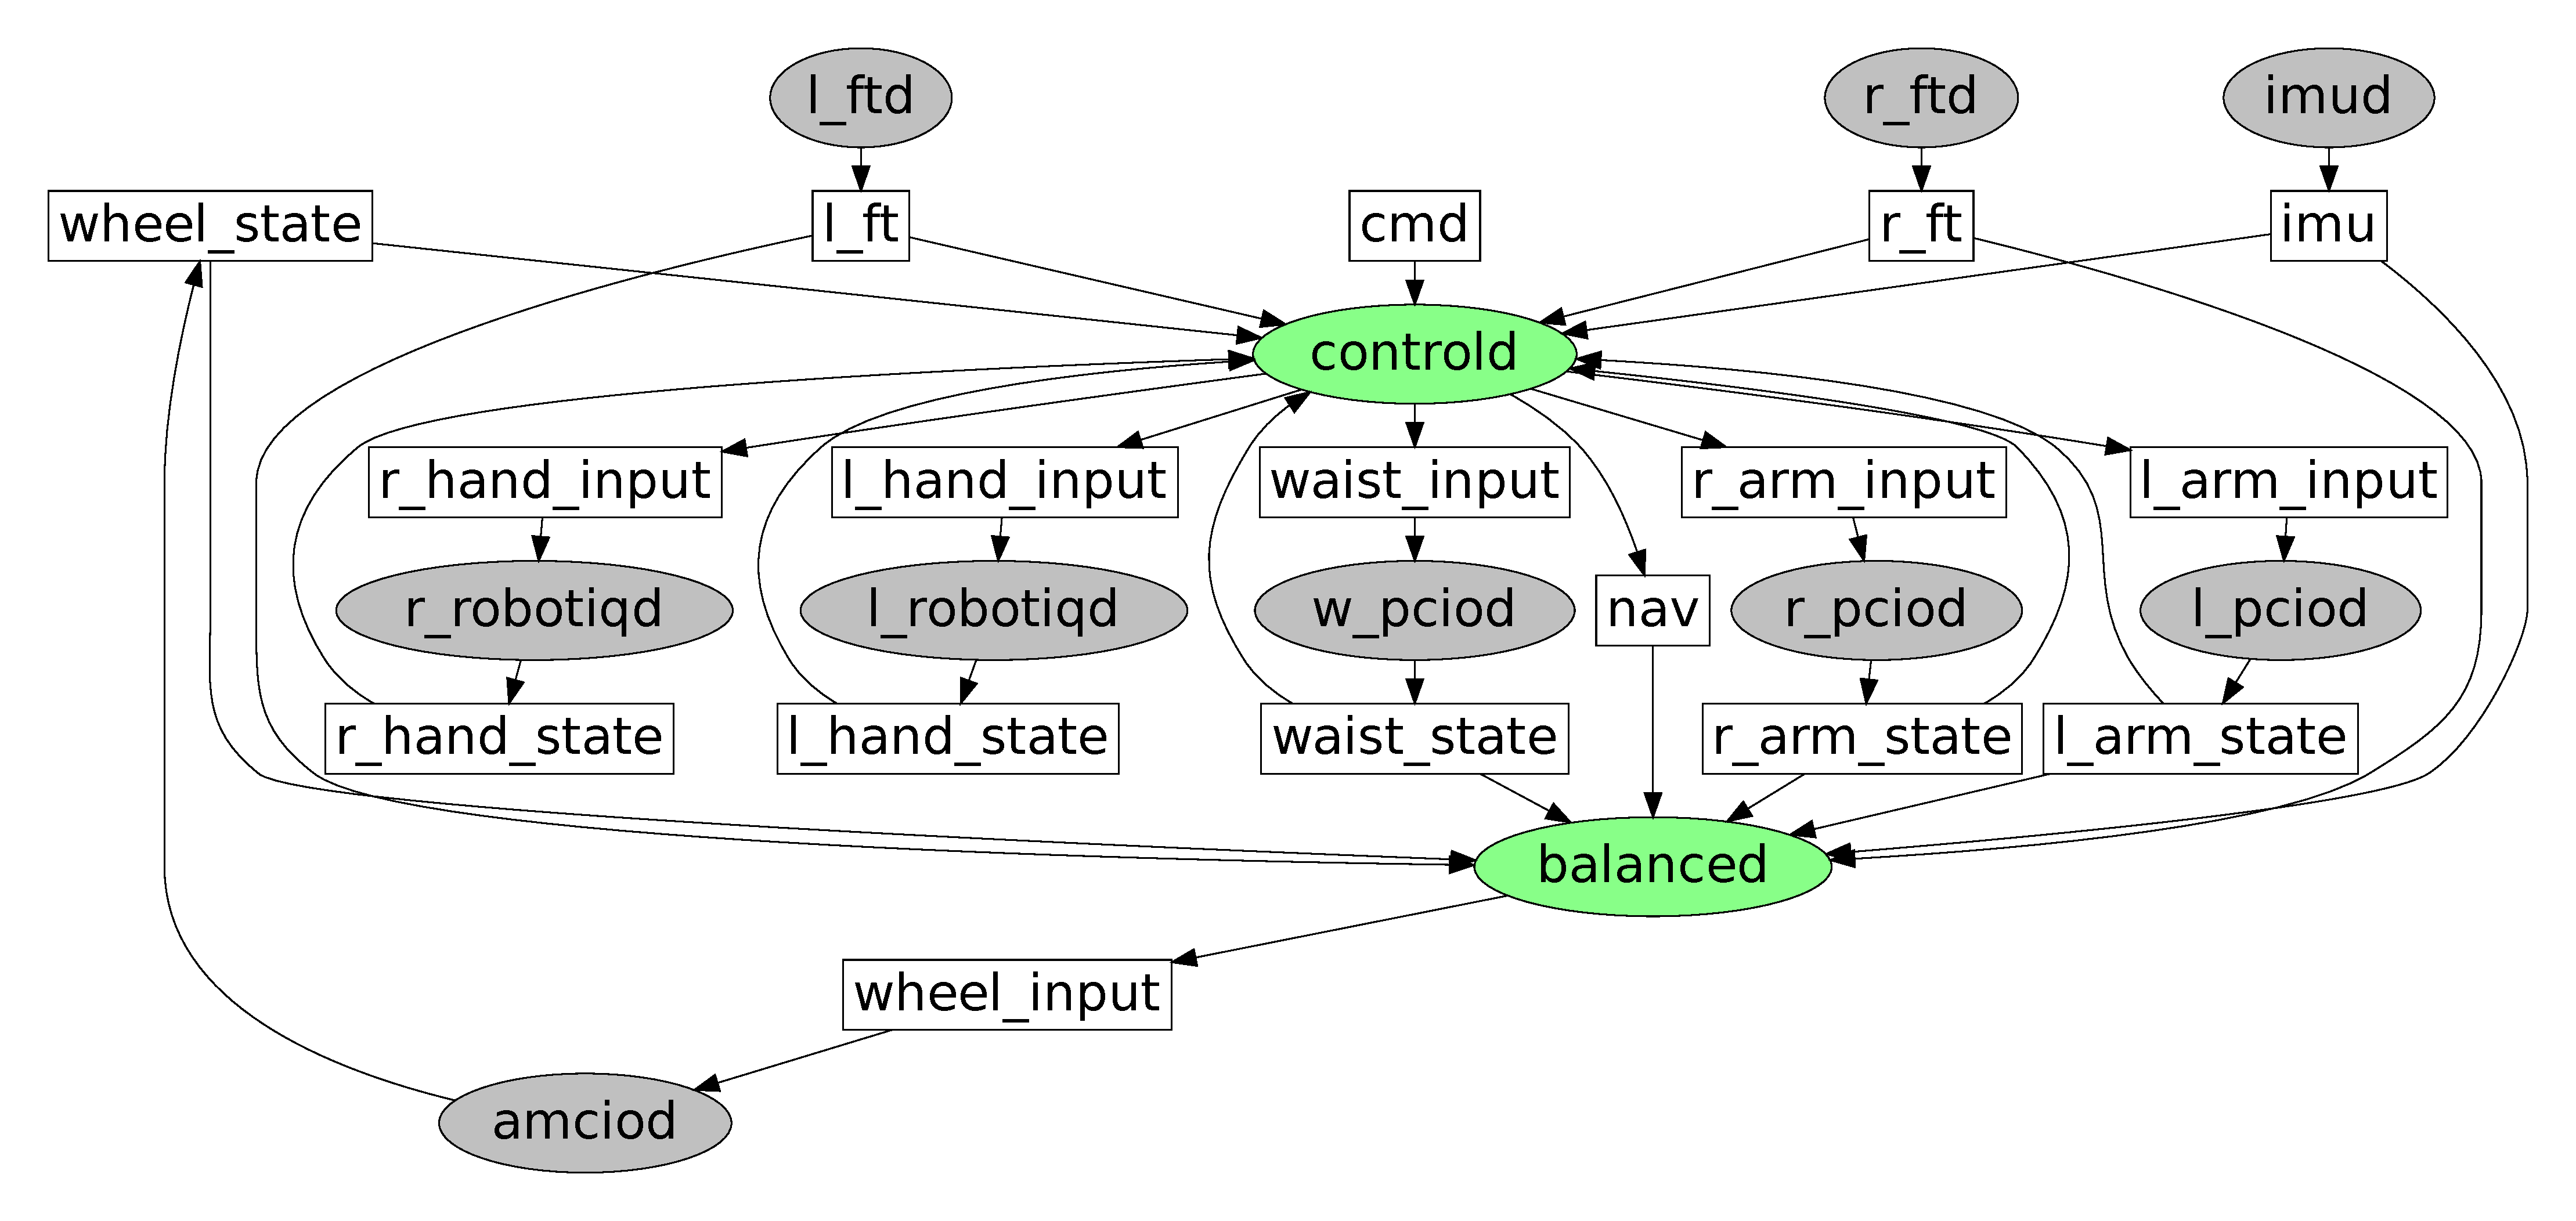
\includegraphics[width=.5\textwidth]{fig/krangdot}
  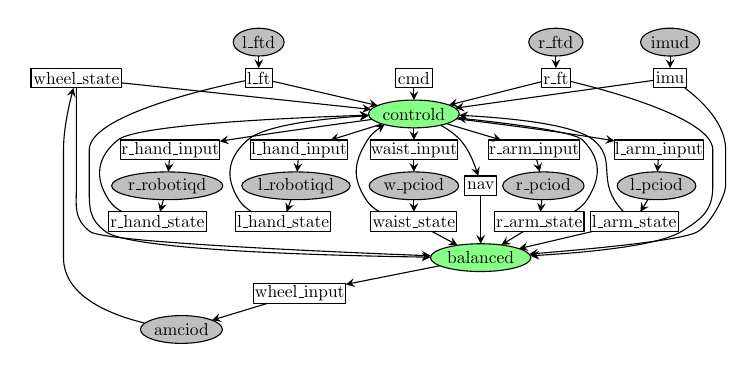
\begin{tikzpicture}[>=stealth,line
    join=bevel,scale=.122,every node/.style={scale=0.63}]
    %%
\pgfsetcolor{black}
  % Edge: ch_l_hand_input -> l_robotiqd
  \draw [->] (788.52bp,541.75bp) .. controls (788.1bp,536.84bp) and (787.65bp,531.59bp)  .. (785.49bp,506.05bp);
  % Edge: ch_l_hand_state -> controld
  \draw [->] (651.86bp,388.16bp) .. controls (636.41bp,397.19bp) and (622.37bp,408.9bp)  .. (613bp,424bp) .. controls (571.33bp,491.2bp) and (579.99bp,547.37bp)  .. (639bp,600bp) .. controls (687.93bp,643.63bp) and (851.77bp,662.6bp)  .. (996.97bp,672.05bp);
  % Edge: ch_r_hand_state -> controld
  \draw [->] (269.01bp,388.14bp) .. controls (253.15bp,397.11bp) and (238.82bp,408.79bp)  .. (229bp,424bp) .. controls (186.07bp,490.48bp) and (194.94bp,549.66bp)  .. (256bp,600bp) .. controls (310.21bp,644.69bp) and (740.24bp,664.96bp)  .. (996.35bp,673.45bp);
  % Edge: l_robotiqd -> ch_l_hand_state
  \draw [->] (767.31bp,424.02bp) .. controls (765.33bp,418.49bp) and (763.28bp,412.77bp)  .. (754.41bp,388.05bp);
  % Edge: ch_waist_state -> controld
  \draw [->] (1028.8bp,388.1bp) .. controls (1013bp,397.09bp) and (998.74bp,408.79bp)  .. (989bp,424bp) .. controls (946.82bp,489.9bp) and (952.06bp,533.32bp)  .. (993bp,600bp) .. controls (1001.4bp,613.65bp) and (1013.1bp,625.09bp)  .. (1043.5bp,645.68bp);
  % Edge: ch_wheel_state -> controld
  \draw [->] (268.07bp,768.73bp) .. controls (454.4bp,748.9bp) and (790.46bp,713.14bp)  .. (1003.2bp,690.49bp);
  % Edge: controld -> ch_waist_input
  \draw [->] (1130bp,635.71bp) .. controls (1130bp,630.71bp) and (1130bp,625.56bp)  .. (1130bp,600.21bp);
  % Edge: ch_imu -> balanced
  \draw [->] (1929.5bp,753.76bp) .. controls (1978.1bp,717.24bp) and (2050bp,649.87bp)  .. (2050bp,571bp) .. controls (2050bp,571bp) and (2050bp,571bp)  .. (2050bp,465bp) .. controls (2050bp,441.6bp) and (2011.6bp,357.89bp)  .. (1968bp,330bp) .. controls (1928.5bp,304.75bp) and (1666.9bp,279.62bp)  .. (1470.3bp,263.62bp);
  % Edge: ch_imu -> controld
  \draw [->] (1837.8bp,776.25bp) .. controls (1725.8bp,760.54bp) and (1444.3bp,721.07bp)  .. (1252bp,694.1bp);
  % Edge: r_ftd -> ch_r_ft
  \draw [->] (1549bp,847.71bp) .. controls (1549bp,842.71bp) and (1549bp,837.56bp)  .. (1549bp,812.21bp);
  % Edge: imud -> ch_imu
  \draw [->] (1886bp,847.71bp) .. controls (1886bp,842.71bp) and (1886bp,837.56bp)  .. (1886bp,812.21bp);
  % Edge: ch_cmd -> controld
  \draw [->] (1130bp,753.75bp) .. controls (1130bp,748.84bp) and (1130bp,743.59bp)  .. (1130bp,718.05bp);
  % Edge: controld -> ch_r_arm_input
  \draw [->] (1226.1bp,648.31bp) .. controls (1269.9bp,635.22bp) and (1322.2bp,619.61bp)  .. (1387.6bp,600.08bp);
  % Edge: controld -> ch_nav
  \draw [->] (1209bp,643.78bp) .. controls (1229.8bp,632.24bp) and (1250.9bp,617.65bp)  .. (1267bp,600bp) .. controls (1289.3bp,575.47bp) and (1304.4bp,541.27bp)  .. (1319.9bp,494.08bp);
  % Edge: ch_r_arm_input -> r_pciod
  \draw [->] (1492.4bp,541.75bp) .. controls (1493.7bp,536.67bp) and (1495.1bp,531.22bp)  .. (1501.5bp,506.05bp);
  % Edge: ch_l_arm_state -> balanced
  \draw [->] (1655.9bp,329.96bp) .. controls (1595.2bp,315.75bp) and (1522bp,298.62bp)  .. (1440.4bp,279.53bp);
  % Edge: ch_r_hand_input -> r_robotiqd
  \draw [->] (408.52bp,541.75bp) .. controls (408.1bp,536.84bp) and (407.65bp,531.59bp)  .. (405.49bp,506.05bp);
  % Edge: r_robotiqd -> ch_r_hand_state
  \draw [->] (390.79bp,424.02bp) .. controls (389.3bp,418.58bp) and (387.76bp,412.96bp)  .. (380.95bp,388.05bp);
  % Edge: ch_l_ft -> controld
  \draw [->] (712.24bp,773.69bp) .. controls (776.67bp,758.77bp) and (905.66bp,728.92bp)  .. (1023.1bp,701.75bp);
  % Edge: ch_r_arm_state -> controld
  \draw [->] (1601.2bp,388.1bp) .. controls (1617bp,397.09bp) and (1631.3bp,408.79bp)  .. (1641bp,424bp) .. controls (1683.3bp,490.06bp) and (1683bp,544.1bp)  .. (1628bp,600bp) .. controls (1603.5bp,624.87bp) and (1416.2bp,648.64bp)  .. (1258.5bp,665.09bp);
  % Edge: ch_nav -> balanced
  \draw [->] (1327bp,435.97bp) .. controls (1327bp,404.75bp) and (1327bp,354.21bp)  .. (1327bp,294.03bp);
  % Edge: ch_waist_input -> w_pciod
  \draw [->] (1130bp,541.75bp) .. controls (1130bp,536.84bp) and (1130bp,531.59bp)  .. (1130bp,506.05bp);
  % Edge: ch_l_arm_input -> l_pciod
  \draw [->] (1851.1bp,541.75bp) .. controls (1850.7bp,536.84bp) and (1850.4bp,531.59bp)  .. (1848.7bp,506.05bp);
  % Edge: balanced -> ch_wheel_input
  \draw [->] (1206.5bp,229.08bp) .. controls (1130.3bp,213.95bp) and (1030.9bp,194.23bp)  .. (929.05bp,174.01bp);
  % Edge: controld -> ch_r_hand_input
  \draw [->] (1006.7bp,660.84bp) .. controls (895.12bp,645.96bp) and (726.36bp,622.8bp)  .. (580bp,600bp) .. controls (578.95bp,599.84bp) and (577.89bp,599.67bp)  .. (557.06bp,596.35bp);
  % Edge: ch_waist_state -> balanced
  \draw [->] (1184.1bp,329.89bp) .. controls (1201.7bp,320.42bp) and (1221.7bp,309.65bp)  .. (1258.9bp,289.62bp);
  % Edge: l_pciod -> ch_l_arm_state
  \draw [->] (1821bp,424.93bp) .. controls (1817.1bp,418.54bp) and (1812.9bp,411.89bp)  .. (1798.2bp,388.23bp);
  % Edge: ch_wheel_state -> balanced
  \draw [->] (134bp,753.85bp) .. controls (134bp,712.98bp) and (134bp,636.33bp)  .. (134bp,571bp) .. controls (134bp,571bp) and (134bp,571bp)  .. (134bp,465bp) .. controls (134bp,402.42bp) and (125.13bp,369.09bp)  .. (174bp,330bp) .. controls (211.84bp,299.73bp) and (849.4bp,271.29bp)  .. (1180.2bp,258.37bp);
  % Edge: ch_r_ft -> controld
  \draw [->] (1505.7bp,772.06bp) .. controls (1446.6bp,757.09bp) and (1338bp,729.63bp)  .. (1233.3bp,703.14bp);
  % Edge: controld -> ch_l_hand_input
  \draw [->] (1036bp,647.61bp) .. controls (994.9bp,634.76bp) and (946.32bp,619.57bp)  .. (883.99bp,600.08bp);
  % Edge: ch_r_ft -> balanced
  \draw [->] (1592.1bp,773.03bp) .. controls (1707.1bp,745.23bp) and (2012bp,662.83bp)  .. (2012bp,571bp) .. controls (2012bp,571bp) and (2012bp,571bp)  .. (2012bp,465bp) .. controls (2012bp,392.14bp) and (1981.2bp,367.99bp)  .. (1919bp,330bp) .. controls (1849.7bp,287.67bp) and (1643.5bp,268.31bp)  .. (1473.7bp,258.54bp);
  % Edge: ch_l_ft -> balanced
  \draw [->] (631.93bp,775.05bp) .. controls (513.28bp,750.37bp) and (172bp,670.71bp)  .. (172bp,571bp) .. controls (172bp,571bp) and (172bp,571bp)  .. (172bp,465bp) .. controls (172bp,401.32bp) and (169.28bp,368.5bp)  .. (220bp,330bp) .. controls (292.9bp,274.66bp) and (867.58bp,259.05bp)  .. (1179bp,254.39bp);
  % Edge: ch_l_arm_state -> controld
  \draw [->] (1749bp,388.04bp) .. controls (1739.1bp,398.62bp) and (1728.6bp,411.15bp)  .. (1721bp,424bp) .. controls (1678.8bp,495.2bp) and (1723.8bp,547.26bp)  .. (1660bp,600bp) .. controls (1604.1bp,646.21bp) and (1419.4bp,664.7bp)  .. (1263.7bp,673.12bp);
  % Edge: r_pciod -> ch_r_arm_state
  \draw [->] (1507.4bp,424.02bp) .. controls (1506.8bp,418.77bp) and (1506.2bp,413.35bp)  .. (1503.3bp,388.05bp);
  % Edge: ch_wheel_input -> amciod
  \draw [->] (697.17bp,117.89bp) .. controls (652.68bp,104.38bp) and (599.55bp,88.245bp)  .. (534.21bp,68.4bp);
  % Edge: l_ftd -> ch_l_ft
  \draw [->] (672bp,847.71bp) .. controls (672bp,842.71bp) and (672bp,837.56bp)  .. (672bp,812.21bp);
  % Edge: ch_r_arm_state -> balanced
  \draw [->] (1452.3bp,329.75bp) .. controls (1437.7bp,320.84bp) and (1421.3bp,310.8bp)  .. (1388.2bp,290.51bp);
  % Edge: amciod -> ch_wheel_state
  \draw [->] (336.27bp,59.746bp) .. controls (234.07bp,84.446bp) and (96bp,138.92bp)  .. (96bp,253bp) .. controls (96bp,571bp) and (96bp,571bp)  .. (96bp,571bp) .. controls (96bp,627.75bp) and (109.35bp,691.72bp)  .. (125.38bp,753.8bp);
  % Edge: w_pciod -> ch_waist_state
  \draw [->] (1130bp,423.71bp) .. controls (1130bp,418.71bp) and (1130bp,413.56bp)  .. (1130bp,388.21bp);
  % Edge: controld -> ch_l_arm_input
  \draw [->] (1255.8bp,662.63bp) .. controls (1368.5bp,649.21bp) and (1538.9bp,627.59bp)  .. (1721.9bp,597.62bp);
  % Node: ch_wheel_state
\begin{scope}
  \definecolor{strokecol}{rgb}{0.0,0.0,0.0};
  \pgfsetstrokecolor{strokecol}
  \draw (268bp,812bp) -- (0bp,812bp) -- (0bp,754bp) -- (268bp,754bp) -- cycle;
  \draw (134bp,783bp) node {wheel\_state};
\end{scope}
  % Node: amciod
\begin{scope}
  \definecolor{strokecol}{rgb}{0.0,0.0,0.0};
  \pgfsetstrokecolor{strokecol}
  \definecolor{fillcol}{rgb}{0.75,0.75,0.75};
  \pgfsetfillcolor{fillcol}
  \filldraw [opacity=1.0] (444bp,41bp) ellipse (121bp and 41bp);
  \draw (444bp,41bp) node {amciod};
\end{scope}
  % Node: balanced
\begin{scope}
  \definecolor{strokecol}{rgb}{0.0,0.0,0.0};
  \pgfsetstrokecolor{strokecol}
  \definecolor{fillcol}{rgb}{0.53,1.0,0.53};
  \pgfsetfillcolor{fillcol}
  \filldraw [opacity=1.0] (1327bp,253bp) ellipse (148bp and 41bp);
  \draw (1327bp,253bp) node {balanced};
\end{scope}
  % Node: ch_l_hand_state
\begin{scope}
  \definecolor{strokecol}{rgb}{0.0,0.0,0.0};
  \pgfsetstrokecolor{strokecol}
  \draw (885bp,388bp) -- (603bp,388bp) -- (603bp,330bp) -- (885bp,330bp) -- cycle;
  \draw (744bp,359bp) node {l\_hand\_state};
\end{scope}
  % Node: w_pciod
\begin{scope}
  \definecolor{strokecol}{rgb}{0.0,0.0,0.0};
  \pgfsetstrokecolor{strokecol}
  \definecolor{fillcol}{rgb}{0.75,0.75,0.75};
  \pgfsetfillcolor{fillcol}
  \filldraw [opacity=1.0] (1130bp,465bp) ellipse (132bp and 41bp);
  \draw (1130bp,465bp) node {w\_pciod};
\end{scope}
  % Node: l_robotiqd
\begin{scope}
  \definecolor{strokecol}{rgb}{0.0,0.0,0.0};
  \pgfsetstrokecolor{strokecol}
  \definecolor{fillcol}{rgb}{0.75,0.75,0.75};
  \pgfsetfillcolor{fillcol}
  \filldraw [opacity=1.0] (782bp,465bp) ellipse (160bp and 41bp);
  \draw (782bp,465bp) node {l\_robotiqd};
\end{scope}
  % Node: imud
\begin{scope}
  \definecolor{strokecol}{rgb}{0.0,0.0,0.0};
  \pgfsetstrokecolor{strokecol}
  \definecolor{fillcol}{rgb}{0.75,0.75,0.75};
  \pgfsetfillcolor{fillcol}
  \filldraw [opacity=1.0] (1886bp,889bp) ellipse (87bp and 41bp);
  \draw (1886bp,889bp) node {imud};
\end{scope}
  % Node: ch_waist_state
\begin{scope}
  \definecolor{strokecol}{rgb}{0.0,0.0,0.0};
  \pgfsetstrokecolor{strokecol}
  \draw (1257bp,388bp) -- (1003bp,388bp) -- (1003bp,330bp) -- (1257bp,330bp) -- cycle;
  \draw (1130bp,359bp) node {waist\_state};
\end{scope}
  % Node: r_ftd
\begin{scope}
  \definecolor{strokecol}{rgb}{0.0,0.0,0.0};
  \pgfsetstrokecolor{strokecol}
  \definecolor{fillcol}{rgb}{0.75,0.75,0.75};
  \pgfsetfillcolor{fillcol}
  \filldraw [opacity=1.0] (1549bp,889bp) ellipse (80bp and 41bp);
  \draw (1549bp,889bp) node {r\_ftd};
\end{scope}
  % Node: ch_r_arm_input
\begin{scope}
  \definecolor{strokecol}{rgb}{0.0,0.0,0.0};
  \pgfsetstrokecolor{strokecol}
  \draw (1619bp,600bp) -- (1351bp,600bp) -- (1351bp,542bp) -- (1619bp,542bp) -- cycle;
  \draw (1485bp,571bp) node {r\_arm\_input};
\end{scope}
  % Node: ch_waist_input
\begin{scope}
  \definecolor{strokecol}{rgb}{0.0,0.0,0.0};
  \pgfsetstrokecolor{strokecol}
  \draw (1258bp,600bp) -- (1002bp,600bp) -- (1002bp,542bp) -- (1258bp,542bp) -- cycle;
  \draw (1130bp,571bp) node {waist\_input};
\end{scope}
  % Node: ch_r_hand_input
\begin{scope}
  \definecolor{strokecol}{rgb}{0.0,0.0,0.0};
  \pgfsetstrokecolor{strokecol}
  \draw (557bp,600bp) -- (265bp,600bp) -- (265bp,542bp) -- (557bp,542bp) -- cycle;
  \draw (411bp,571bp) node {r\_hand\_input};
\end{scope}
  % Node: r_robotiqd
\begin{scope}
  \definecolor{strokecol}{rgb}{0.0,0.0,0.0};
  \pgfsetstrokecolor{strokecol}
  \definecolor{fillcol}{rgb}{0.75,0.75,0.75};
  \pgfsetfillcolor{fillcol}
  \filldraw [opacity=1.0] (402bp,465bp) ellipse (164bp and 41bp);
  \draw (402bp,465bp) node {r\_robotiqd};
\end{scope}
  % Node: controld
\begin{scope}
  \definecolor{strokecol}{rgb}{0.0,0.0,0.0};
  \pgfsetstrokecolor{strokecol}
  \definecolor{fillcol}{rgb}{0.53,1.0,0.53};
  \pgfsetfillcolor{fillcol}
  \filldraw [opacity=1.0] (1130bp,677bp) ellipse (134bp and 41bp);
  \draw (1130bp,677bp) node {controld};
\end{scope}
  % Node: ch_imu
\begin{scope}
  \definecolor{strokecol}{rgb}{0.0,0.0,0.0};
  \pgfsetstrokecolor{strokecol}
  \draw (1934bp,812bp) -- (1838bp,812bp) -- (1838bp,754bp) -- (1934bp,754bp) -- cycle;
  \draw (1886bp,783bp) node {imu};
\end{scope}
  % Node: ch_l_arm_state
\begin{scope}
  \definecolor{strokecol}{rgb}{0.0,0.0,0.0};
  \pgfsetstrokecolor{strokecol}
  \draw (1910bp,388bp) -- (1650bp,388bp) -- (1650bp,330bp) -- (1910bp,330bp) -- cycle;
  \draw (1780bp,359bp) node {l\_arm\_state};
\end{scope}
  % Node: ch_r_ft
\begin{scope}
  \definecolor{strokecol}{rgb}{0.0,0.0,0.0};
  \pgfsetstrokecolor{strokecol}
  \draw (1592bp,812bp) -- (1506bp,812bp) -- (1506bp,754bp) -- (1592bp,754bp) -- cycle;
  \draw (1549bp,783bp) node {r\_ft};
\end{scope}
  % Node: ch_r_arm_state
\begin{scope}
  \definecolor{strokecol}{rgb}{0.0,0.0,0.0};
  \pgfsetstrokecolor{strokecol}
  \draw (1632bp,388bp) -- (1368bp,388bp) -- (1368bp,330bp) -- (1632bp,330bp) -- cycle;
  \draw (1500bp,359bp) node {r\_arm\_state};
\end{scope}
  % Node: l_ftd
\begin{scope}
  \definecolor{strokecol}{rgb}{0.0,0.0,0.0};
  \pgfsetstrokecolor{strokecol}
  \definecolor{fillcol}{rgb}{0.75,0.75,0.75};
  \pgfsetfillcolor{fillcol}
  \filldraw [opacity=1.0] (672bp,889bp) ellipse (75bp and 41bp);
  \draw (672bp,889bp) node {l\_ftd};
\end{scope}
  % Node: ch_cmd
\begin{scope}
  \definecolor{strokecol}{rgb}{0.0,0.0,0.0};
  \pgfsetstrokecolor{strokecol}
  \draw (1184bp,812bp) -- (1076bp,812bp) -- (1076bp,754bp) -- (1184bp,754bp) -- cycle;
  \draw (1130bp,783bp) node {cmd};
\end{scope}
  % Node: ch_nav
\begin{scope}
  \definecolor{strokecol}{rgb}{0.0,0.0,0.0};
  \pgfsetstrokecolor{strokecol}
  \draw (1374bp,494bp) -- (1280bp,494bp) -- (1280bp,436bp) -- (1374bp,436bp) -- cycle;
  \draw (1327bp,465bp) node {nav};
\end{scope}
  % Node: ch_wheel_input
\begin{scope}
  \definecolor{strokecol}{rgb}{0.0,0.0,0.0};
  \pgfsetstrokecolor{strokecol}
  \draw (929bp,176bp) -- (657bp,176bp) -- (657bp,118bp) -- (929bp,118bp) -- cycle;
  \draw (793bp,147bp) node {wheel\_input};
\end{scope}
  % Node: l_pciod
\begin{scope}
  \definecolor{strokecol}{rgb}{0.0,0.0,0.0};
  \pgfsetstrokecolor{strokecol}
  \definecolor{fillcol}{rgb}{0.75,0.75,0.75};
  \pgfsetfillcolor{fillcol}
  \filldraw [opacity=1.0] (1846bp,465bp) ellipse (116bp and 41bp);
  \draw (1846bp,465bp) node {l\_pciod};
\end{scope}
  % Node: ch_r_hand_state
\begin{scope}
  \definecolor{strokecol}{rgb}{0.0,0.0,0.0};
  \pgfsetstrokecolor{strokecol}
  \draw (517bp,388bp) -- (229bp,388bp) -- (229bp,330bp) -- (517bp,330bp) -- cycle;
  \draw (373bp,359bp) node {r\_hand\_state};
\end{scope}
  % Node: r_pciod
\begin{scope}
  \definecolor{strokecol}{rgb}{0.0,0.0,0.0};
  \pgfsetstrokecolor{strokecol}
  \definecolor{fillcol}{rgb}{0.75,0.75,0.75};
  \pgfsetfillcolor{fillcol}
  \filldraw [opacity=1.0] (1512bp,465bp) ellipse (120bp and 41bp);
  \draw (1512bp,465bp) node {r\_pciod};
\end{scope}
  % Node: ch_l_arm_input
\begin{scope}
  \definecolor{strokecol}{rgb}{0.0,0.0,0.0};
  \pgfsetstrokecolor{strokecol}
  \draw (1984bp,600bp) -- (1722bp,600bp) -- (1722bp,542bp) -- (1984bp,542bp) -- cycle;
  \draw (1853bp,571bp) node {l\_arm\_input};
\end{scope}
  % Node: ch_l_ft
\begin{scope}
  \definecolor{strokecol}{rgb}{0.0,0.0,0.0};
  \pgfsetstrokecolor{strokecol}
  \draw (712bp,812bp) -- (632bp,812bp) -- (632bp,754bp) -- (712bp,754bp) -- cycle;
  \draw (672bp,783bp) node {l\_ft};
\end{scope}
  % Node: ch_l_hand_input
\begin{scope}
  \definecolor{strokecol}{rgb}{0.0,0.0,0.0};
  \pgfsetstrokecolor{strokecol}
  \draw (934bp,600bp) -- (648bp,600bp) -- (648bp,542bp) -- (934bp,542bp) -- cycle;
  \draw (791bp,571bp) node {l\_hand\_input};
\end{scope}
%
  \end{tikzpicture}
  \caption{Block diagram of primary software components on Golem
    Krang. Gray ovals are user-space driver processes, green ovals are
    controller processes, and rectangles are Ach channels.}
  \label{fig:krangsoft}
  \vspace{-2.0em}
\end{figure}

The software for Krang is implemented as a collection of processes
communicating over Ach channels, \autoref{fig:krangsoft}.  Each
hardware device, such as the IMU or an LWA3 arm, is managed by a
userspace driver daemon.  These drivers are independent operating
system processes that initialize the hardware, then read state and
send commanded control inputs to hardware device.  These state and
input messages flow through a variety of ach channels.  State messages
include values such as positions, velocities, and forces.  Input
messages include values such as reference velocities or voltages. Each
driver daemon has one channel for the device state messages, ensuring
that the current state of the robot can always be accessed as the
newest message in each of these channels.  Devices that take an input
command have a second channel for that input.  In addition to the
driver daemons, there are two controller daemon processes.  The {\tt
  balanced} process implements the stable balancing controller for
Krang.  Control of the arms and reference forward and rotational
speeds are handled in the separate {\tt controld} process.  Dividing
these controllers promotes robustness by isolating the highly-critical
balance control from other faults.  This collection of driver and
controller daemons communicating over Ach channels implements the
real-time, kilohertz control loop for Golem Krang.

This design produces a system that is efficient, modular, and robust.
The low overhead and suitable semantics of Ach communication permits
real-time control under Linux using multiple processes. In several
cases, Krang contains multiple identical hardware devices.  The
message-passing, multi-process design aids code reuse by allowing
access to duplicated devices with multiple instances of the same
daemon binary -- two instances of the ftd daemon for the F/T sensors,
two instances of the robotiqd daemon for the grippers, and three
instances of the pciod daemon for two arms and torso.  The relative
independence of each running process makes this system robust to
failures in non-critical components.  For example, an electrical
failure in a waist motor may stall the w\_pciod process, but --
without any additional code -- the balanced controller and amciod
driver daemons continue running independently, ensuring that the robot
does not fall.  Thus, Ach helps enhance the safety of this potentially
dangerous robotic system.


% Added a section of NAO software implementation.
\subsection{Speed Regulation on NAO}

\label{sec:nao_walking}

%An approach to control the walking speed of NAO was achieved by
%using the Human-Inspired Control (HIC) and Context-Free Motion Grammar (CFG).

The NAO is a small bipedal robot produced by Aldebaran Robotics.  It
contains an on-board Intel Atom PC running a minimal Linux
distribution and includes the NAOqi framework to control the robot.
User code is loaded into the NAOqi process as dynamic library modules.
We used Ach to implement Human-Inspired Control \cite{Ames:NAO:2012}
on the NAO.  The Human-Inspired Control approach achieves provably
stable, human-like walking on robots by identifying key parameters in
human gaits, and transferring those to the robot through an
optimization process \cite{Ames11}.  To implement this approach,
real-time control software to produce the desired joint angles must
run on the NAO's internal computer.

% speed based on theoretically stable periodic orbits. The
% Human-Inspired Control provides a set of control parameters to
% generate the joint trajectories for stable walking with a certain
% fixed walking speed.

The NAOqi framework provides an interface to the robot's hardware;
however, it presents some specific challenges for application
development -- and for the implementation of Human-Inspired Control in
particular.  NAOqi is slow and memory-intensive, consuming at idle
15\% of available CPU time and 20\% of available memory.
Additionally, real-time user code must run as a callback function,
which is awkward for the desired controller implementation.  Using Ach
to move the controller to a separate process improves the
implementation.


A multi-process software design, \autoref{fig:naoprogram}, addresses
the shortcomings of NAOqi. In this approach, two separate processes,
{\tt motionControl} and {\tt logger/debugger}, interface with NAOqi
through the Ach IPC library. Two Ach channels are used: a control
channel for command data from {\tt motionControl} and a feedback
channel for sensor data from NAOqi. In order connect NAOqi with these
other processes via Ach, a minimal local module, {\tt libamber}, loads
into the NAOqi process, and all nonessential modules of NAOqi are
deactivated.  The {\tt libamber} module communicates over the two Ach
channels using the periodic, 10ms callback function provided by the
NAO's Device Communication Manager (DCM). When the DCM reads a new set
of sensor values, it notifies {\tt libamber} using a post-process
callback function. After that, {\tt libamber} writes the newly-read
sensor values into the feedback channel.  Before the DCM transmits
desired actuator values to the hardware, it calls a pre-process
callback function. On this event, {\tt libamber} reads the newest
command values from the control channel and then sends it to NAO's
servomotors through the DCM.

The {\tt motionControl} process produces the desired angles for
human-like walking on NAO. This process contains two core modules,
{\tt motionParser} and {\tt trajectoryGenerator}. The {\tt
  motionParser} \cite{dantam2013tro} contains a Finite State Machine
(FSM) which parses the robot's current state based on the newest
sensor data read from the feedback channel. Then {\tt
  trajectoryGenerator} computes the desired joint angles to yield
human-like walking on the NAO \cite{jars_2012_psa_01}.

The {\tt logger/debugger} process records data from both Ach
channels. This shows robot state during operation and allows offline
analysis of the data.  Since this process runs at lower priority than
both {\tt motionControl} and NAOqi, it does not affects the real-time
control of the robot.

In addition to steady-state fixed speed walking, we implement
speed-controlled walking on the NAO by tracking a stable sequence of
speed transitions. The {\tt Supervisor Generator} process computes a
\emph{supervisor} for a stable path of transitions to the desired
speed, adjusting the behavior of the {\tt motionParser}.  These two
processes communicate over two Ach channels: {\tt chan\_vel} contains
the current walking speed of the robot at the end of each step, and
{\tt chan\_super} contains the active supervisor for the target speed.


Adopting this multi-process design based on the Ach IPC library
enhances the robustness and efficiency of Human-Inspired Control on
the NAO.  Each process runs independently, so an error in a
non-critical process, such as {\tt logger/debugger}, cannot affect
other processes, eliminating a potential failure.  The user processes
can be stopped and started within only a few seconds.  In contrast,
NAOqi takes about 15 seconds to start. The independence of processes
means NAOqi need not be restarted so long as {\tt libamber} is
unchanged.  Since {\tt libamber} is a minimal module, only interfacing
with the Ach channels and accessing the NAO's hardware, it can be
reused unmodified for different applications on the NAO. Different
projects can run different controller processes, using Ach and {\tt
  libamber} to access NAO's hardware, all without restarting the NAOqi
process.  In addition, using standard debugging tools such as GDB is
much easier since the user code can be executed within the debugger
independently of the NAOqi framework.  Thus, converting the NAO's
control software to a multi-process design simplified development and
improved reliability.



\begin{figure}
  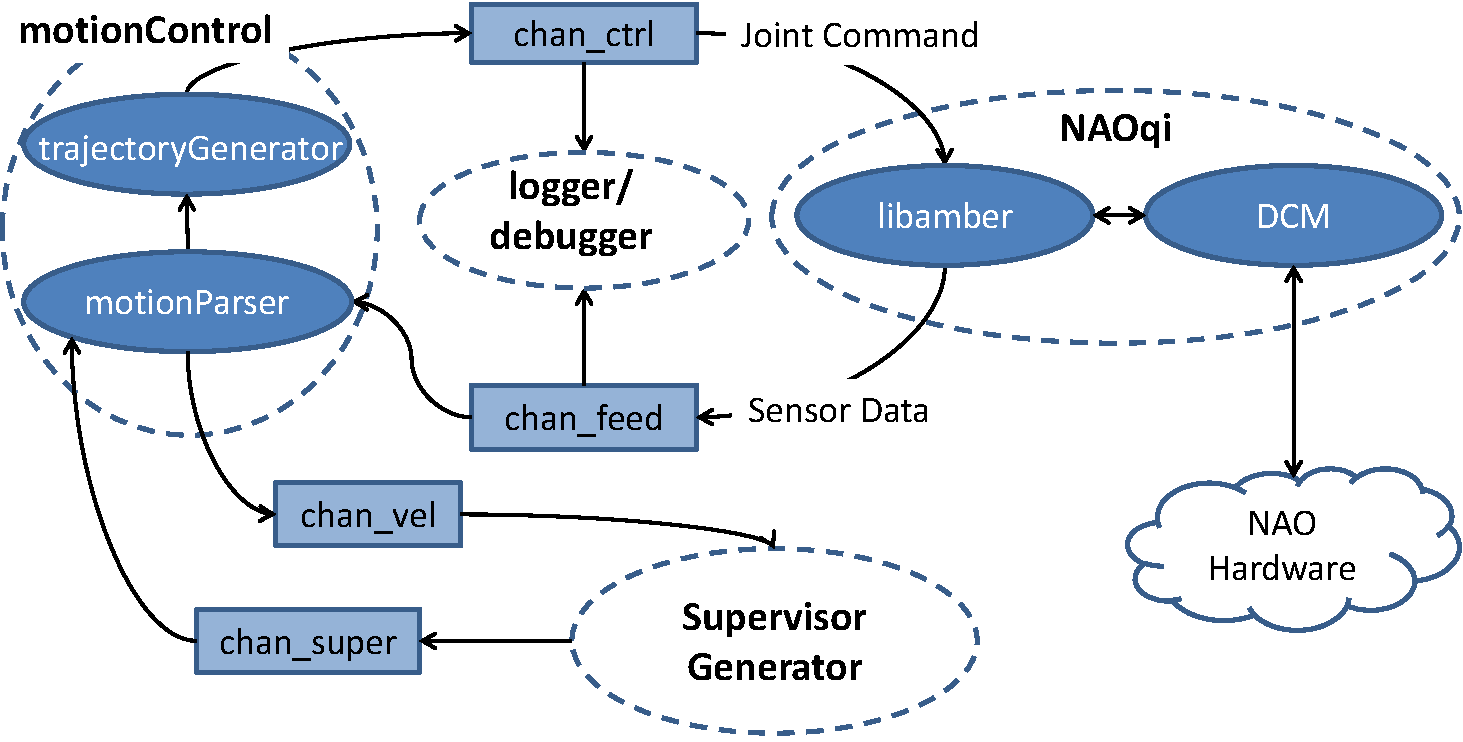
\includegraphics[width=.5\textwidth]{fig/naoprogram}
  \caption{Block diagram of primary software components on NAO.
  Ovals with dashed line are system processes, blue ovals with solid
line are modules contain within process, and rectangles are Ach channels.}
  \label{fig:naoprogram}
  \vspace{-2.0em}
\end{figure}

%%% Local Variables:
%%% mode: latex
%%% TeX-master: "ach.tex"
%%% End:


\subsection{HUBO 2 Plus}
\section{Hubo2 Plus}
Hubo2 Plus, Hubo for short, is a 130 $cm$ (4' 3'') tall, 42 $kg$ (93 $lb$) full-size humanoid robot.  
It was designed and constructed by Prof Jun-Ho Oh and the Hubo Lab at the Korean Advanced Institute of Science and Technology\cite{hubo-first}.
Hubo has 2 arms, 2 legs and a head, making it anthropomorphic to a human.  
It boasts 38 degrees of freedom (DOF) consisting of 6x in each leg, 6x in each arm, 5x in each hand, 3x in the neck, and 1x in the waist.
All joints with the exception of the fingers are high gain PD position controlled.
The fingers are PWM controlled.
It has a three axis force torque (FT) sensor on leg between the end of the ankle and the foot and on the arm where it connects to the hand.
Additionally it has accelerometers on each foot and a six axis inertial measurement unit (IMU) slightly below it's weight (approximately the centre of mass).
The reference commands for all of the joints are sent from the primary control computer (x86) to the individual motor controllers via two Controller Area Network (CAN) buses.
There are currently eight Hubo's functioning in the United States as of December 2012.
Four reside at Drexel University and one at Georgia Tech, Perdue, Ohio State and MIT.
Jaemi Hubo is the oldest of the Hubos in America and has been at the Drexel Autonomous Systems Lab\footnote{Drexel Autonomous Systems Lab: http://dasl.mem.drexel.edu/} (DASL) since 2008\cite{jaemiHuboSRM}.
Fig.~\ref{fig:hubo} shows the major dimensions of Hubo.

\begin{figure}[thpb]
  \centering
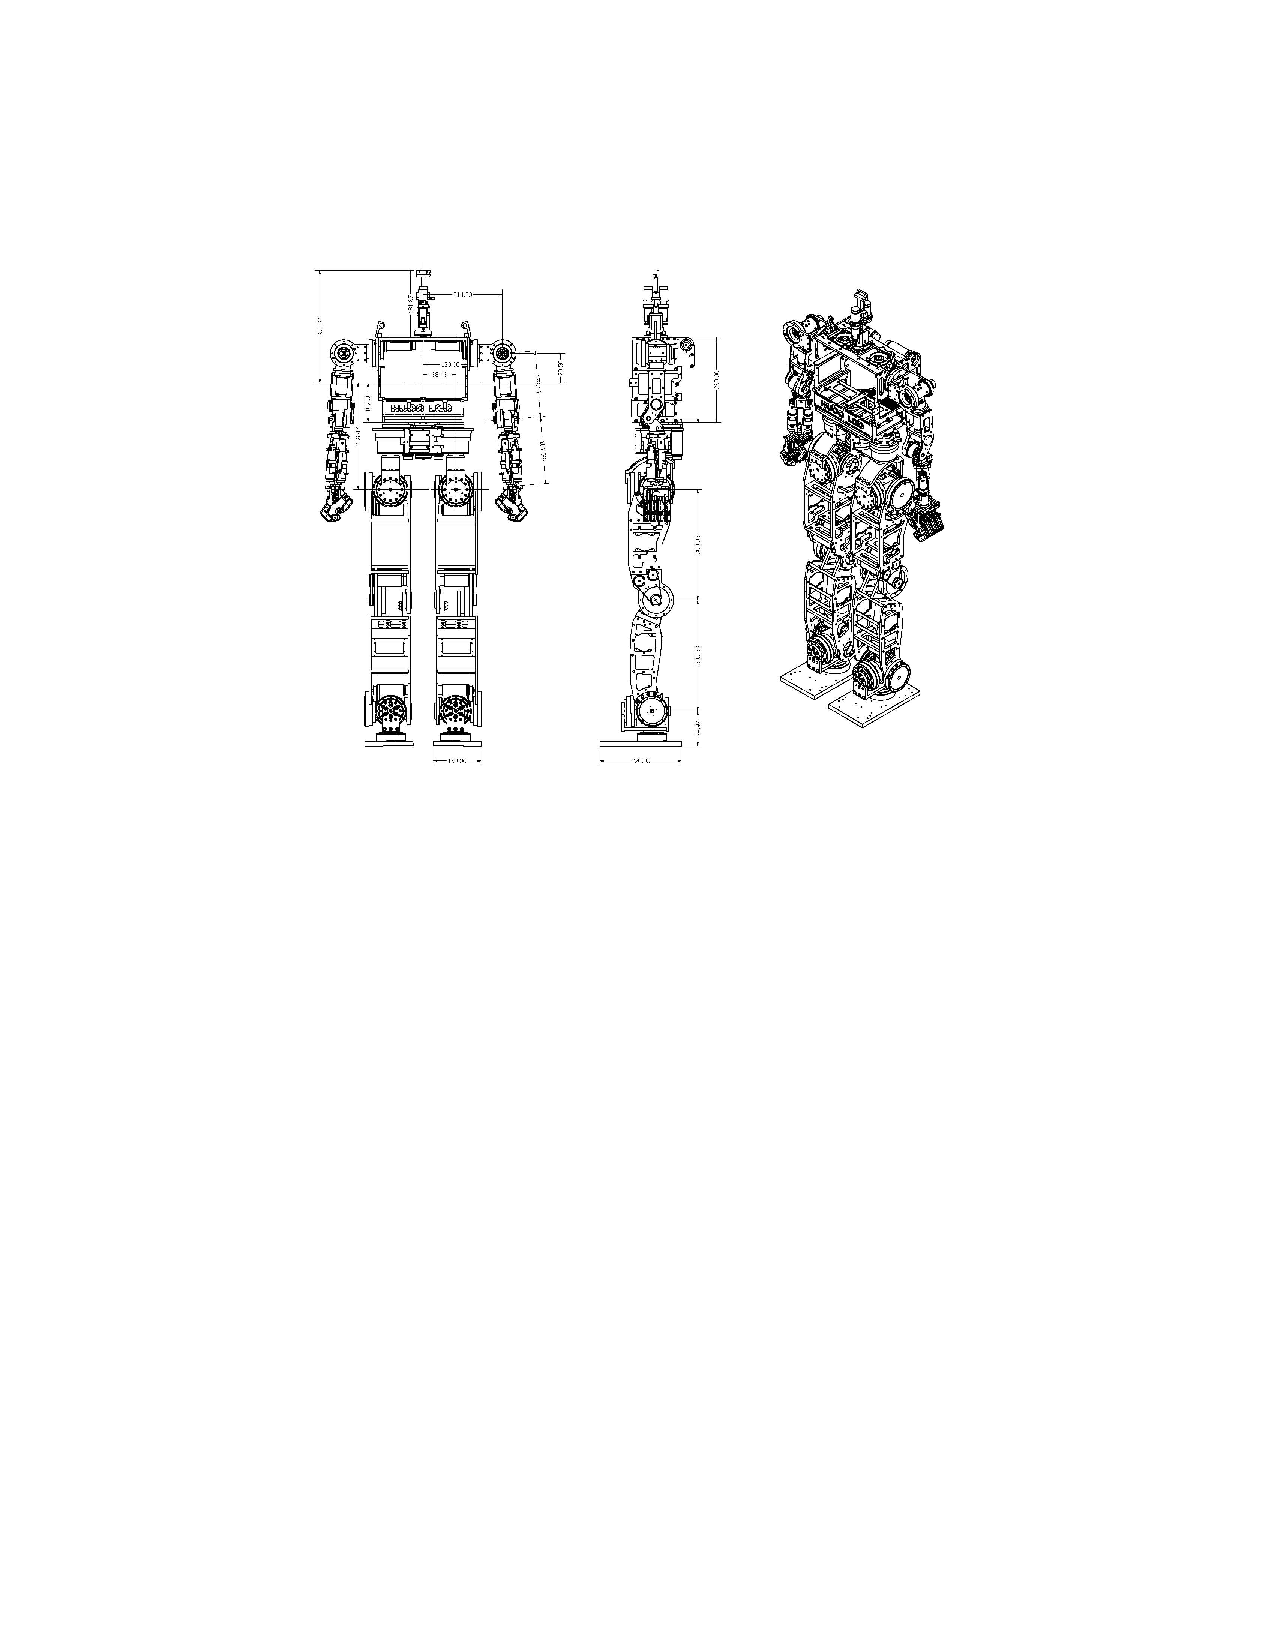
\includegraphics[width=1.0\columnwidth]{./pix/huboSkel.pdf}
  \caption{Hubo2 platform: 130 $cm$ tall full-size humanoid robot weighing 37 $kg$.  It has 38 DOF consisting of 6x in each leg, 6x in each arm, 5x in each hand, 1x in the waist, and 3x in the neck.}
  \label{fig:hubo}
\end{figure}





\section{Verification, Benchmarks, and Discussion}
\label{sect:vb}
\subsection{Formal Verification}

We used the SPIN Model Checker \cite{holtzman2004spin} to formally
verify Ach.  Formal verification is a method to enhance the
reliability of software by first \emph{modeling} the operation of that
software and then \emph{checking} that the model adheres to some
specification for performance. SPIN models concurrent programs using
the Promela language.  Then, it enumerates all possible world states
of that model and ensures that each state satisfies the given
specification.

We verified the {\tt ach\_put} and {\tt ach\_get} procedures
using SPIN.  Our model for Ach checks the consistency of channel data
structures, ensures proper transmission of message data, and verifies
freedom from deadlock.  Because model checking enumerates all possible
world states, we can verify these properties for all possible
interleavings of {\tt ach\_put} and {\tt ach\_get}, something that is
practically impossible to achieve through testing alone.  By modeling
the behavior of Ach in Promela and verifying its performance with
SPIN, we eliminated errors in the returned status codes and simplified
our implementation.  Verification enhanced both the robustness and
simplicity of Ach.


\subsection{Benchmarks}

\begin{figure*}
  \def\figw{.23\textwidth}
  % \begin{minipage}[b]{.5\linewidth}
  \subfigure[Pipe 1s/1r]{
    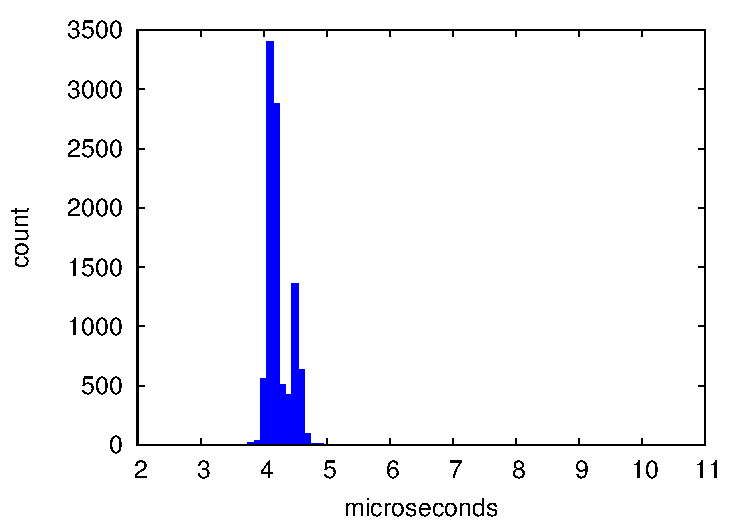
\includegraphics[width=\figw]{plot/calvin-ht-2012-11-11/ach-bench-f1000-s10-P}
  }
  \subfigure[Ach 1s/1r]{
    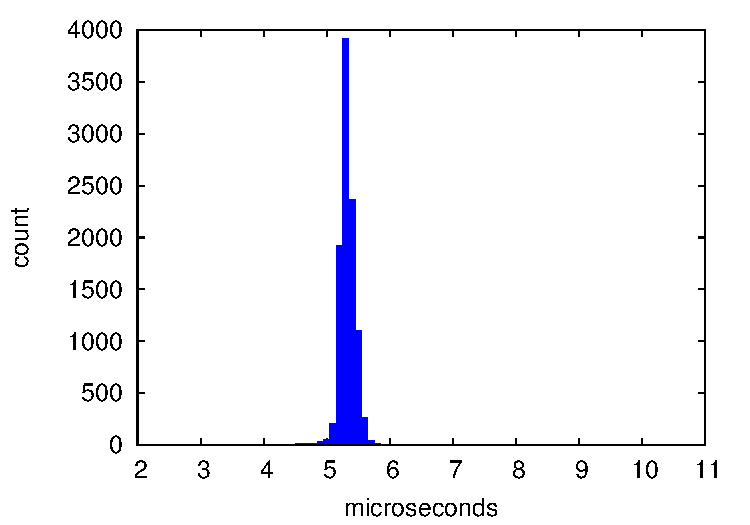
\includegraphics[width=\figw]{plot/calvin-ht-2012-11-11/ach-bench-f1000-s10-p1-r1}
  }
  \subfigure[Ach 1s/2r]{
    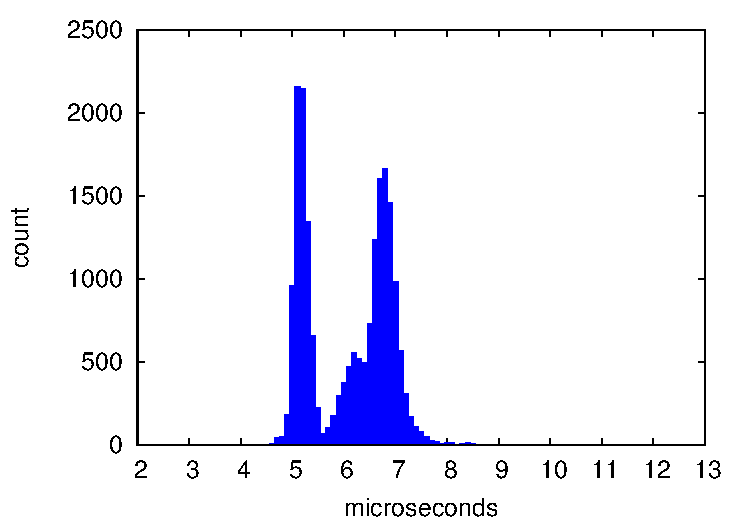
\includegraphics[width=\figw]{plot/calvin-ht-2012-11-11/ach-bench-f1000-s10-p1-r2}
  }
  \subfigure[Ach 2s/2r]{
    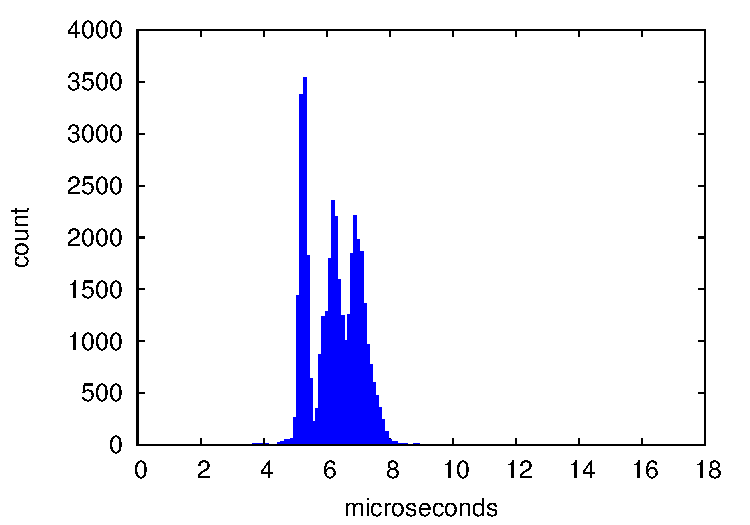
\includegraphics[width=\figw]{plot/calvin-ht-2012-11-11/ach-bench-f1000-s10-p2-r2}
  }
  % \subfigure[Pipe 1s/1r $1 \kilo\hertz$] {
  %   \includegraphics[width=\figw]{bench/daneel-pipe-1k}
  % }\hfil
  % \subfigure[Ach 1s/1r $1 \kilo\hertz$] {
  %   \includegraphics[width=\figw]{bench/daneel-f1000-s4-p1-r1-l0}
  % }\hfil
  % %
  % \subfigure[Pipe 1s/1r $8 \kilo\hertz$] {
  %   \includegraphics[width=\figw]{bench/daneel-pipe-8k}
  % }\hfil
  % \subfigure[Ach  1s/1r $8 \kilo\hertz$] {
  %   \includegraphics[width=\figw]{bench/daneel-f8000-s4-p1-r1-l0}
  % }\hfil
  % %
  % \subfigure[Ach 1s/2r $1 \kilo\hertz$] {
  %   \includegraphics[width=\figw]{bench/daneel-f1000-s4-p1-r2-l0}
  % }\hfil
  % \subfigure[Ach 2s/2r $1 \kilo\hertz$] {
  %   \includegraphics[width=\figw]{bench/daneel-f1000-s4-p2-r2-l0}
  % }\hfil
  % %
  % \subfigure[Ach 4s/4r $1 \kilo\hertz$] {
  %   \includegraphics[width=\figw]{bench/daneel-f1000-s4-p4-r4-l0}
  % }\hfil
  % \subfigure[Ach 1s/8r $1 \kilo\hertz$] {
  %   \includegraphics[width=\figw]{bench/daneel-f1000-s4-p1-r8-l0}
  % }\hfil
  % \subfigure[Ach 1s/2r $8 \kilo\hertz$] {
  %   \includegraphics[width=\figw]{bench/daneel-f8000-s4-p1-r2-l0}
  % }\hfil
  % \subfigure[Ach 2s/2r $8 \kilo\hertz$] {
  %   \includegraphics[width=\figw]{bench/daneel-f8000-s4-p2-r2-l0}
  % }\hfil
  % %
  % \subfigure[Ach 4s/4r $8 \kilo\hertz$] {
  %   \includegraphics[width=\figw]{bench/daneel-f8000-s4-p4-r4-l0}
  % }\hfil
  % \subfigure[Ach 1s/8r $8 \kilo\hertz$] {
  %   \includegraphics[width=\figw]{bench/daneel-f8000-s4-p1-r8-l0}
  % }\hfil
  %\caption{Histograms of pipe messaging latencies.}
  \caption{Histograms of Ach and Pipe messaging latencies.
    Benchmarking performed on a Xeon E3-1270v2 running Linux 3.4.18
    PREEMPT\_RT. The labels $\alpha$s/$\beta$r indicate a test run with
    $\alpha$ sending processes and $\beta$ receiving processes. }
  %\label{fig:bench1}
  \label{fig:bench1}
%\end{minipage}
  \vspace{-15pt}
\end{figure*}




% \begin{figure*}
% \def\figw{.23\textwidth}
% %\begin{minipage}[b]{.5\linewidth}
%   \subfigure[daneel  ach $1 \kilo\hertz$] {
%     \includegraphics[width=\figw]{ach-hist-1k-linux}
%   }\hfil
%   \subfigure[daneel  ach $8 \kilo\hertz$] {
%     \includegraphics[width=\figw]{ach-hist-8k-linux}
%   }\hfil
%   %
%   \subfigure[daneel  pipe $1 \kilo\hertz$] {
%     \includegraphics[width=\figw]{pipe-hist-1k-linux}
%   }\hfil
%   \subfigure[daneel  pipe $8 \kilo\hertz$] {
%     \includegraphics[width=\figw]{pipe-hist-8k-linux}
%   }\hfil
%   %
%   \subfigure[daneel PREEMPT ach $1 \kilo\hertz$] {
%     \includegraphics[width=\figw]{ach-hist-1k-preempt}
%   }\hfil
%   \subfigure[daneel PREEMPT ach $8 \kilo\hertz$] {
%     \includegraphics[width=\figw]{ach-hist-8k-preempt}
%   }\hfil
%   %
%   \subfigure[daneel PREEMPT pipe $1 \kilo\hertz$] {
%     \includegraphics[width=\figw]{pipe-hist-1k-preempt}
%   }\hfil
%   \subfigure[daneel PREEMPT pipe $8 \kilo\hertz$] {
%     \includegraphics[width=\figw]{pipe-hist-8k-preempt}
%   }\hfil
%   %
%   \subfigure[nibbler ach $1 \kilo\hertz$] {
%     \includegraphics[width=\figw]{ach-hist-1k-arm}
%   }\hfil
%   \subfigure[nibbler ach $8 \kilo\hertz$] {
%     \includegraphics[width=\figw]{ach-hist-8k-arm}
%   }\hfil
%   %
%   \subfigure[nibbler pipe $1 \kilo\hertz$] {
%     \includegraphics[width=\figw]{pipe-hist-1k-arm}
%   }\hfil
%   \subfigure[nibbler pipe $8 \kilo\hertz$] {
%     \includegraphics[width=\figw]{pipe-hist-8k-arm}
%   }\hfil
%   %\caption{Histograms of pipe messaging latencies.}
%   \caption{Histograms of Ach and Pipe messaging latencies.  Daneel is a Core 2
%     Duo running Ubuntu Linux 10.04.  The PREEMPT version used the
%     RT\_PREEMPT kernel patch.  Nibbler is an $800 \mega\hertz$ ARM CPU
%     running Debian GNU/Linux 6.0.}
%   %\label{fig:bench1}
%   \label{fig:bench1}
% %\end{minipage}
% \end{figure*}

We provide benchmark results for Ach message latencies in
\autoref{fig:bench1} and include latencies for message sent overs POSIX
pipes as a comparison.

% \subsubsection{Benchmark Platforms}
% The benchmark data was collected on the following platforms:
% \begin{itemize}
%   %\item daneel: Intel Core 2 Duo E7300, Ubuntu Linux 10.04 i386, Kernel
%     %2.6.32-33-generic
%   \item daneel: Intel Core 2 Duo E7300, Ubuntu Linux 10.04 i386,
%     Kernel 2.6.31-11-rt
%   \item nibbler: Qualcomm MSM7230 Snapdragon 800 MHz, Debian GNU/Linux
%     6.0 armel, Kernel 2.6.32.28-cyanogenmod-g4f4ee2e
%   \item natesh: Intel Core i7-2600 3.40GHz, Ubuntu Linux 10.04 x86\_64,
%     Kernel 2.6.32-39-preempt
% \end{itemize}

\subsubsection{Benchmark Procedure}
We perform the benchmarks on an Intel Xeon 1270v2 running Linux Kernel
3.4.18 PREEMPT\_RT.  The benchmark application performs the following
steps.
\begin{enumerate}
  \item Create and open an Ach channel
  \item Fork one or more receiver processes
  \item Fork one or more sender processes
  \item Senders: Post timestamped messages at the desired frequency
  \item Receivers: Receive messages and record latency of each
    messaged based on the timestamp.
\end{enumerate}
We repeat this procedure, varying the frequency and number of senders
and receivers.  The benchmark code is included with the Ach source
distribution.

\subsubsection{Benchmark Results}

These benchmark results in \autoref{fig:bench1} show that Ach first
matches the performance of POSIX pipes for the single sender/receiver
case while also providing non-HOL-blocking semantics and allowing
multiple senders and receivers.  The first two histograms
\autoref{fig:bench1} shows essentially identical performance between
POSIX pipes and single sender and receiver Ach.  This is expected
because the majority of latency should come from the process
context-switch which must occur with both pipes and Ach.  This also
indicates that the cost of the context switch is significantly greater
than the cost of the data copy for the small messages sizes typical of
real-time applications.  The next two plots show Ach performance for
multiple senders and receivers.  The additional processes increase
latency because channel access is restricted to one process at a time.
These results show that the latency imposed by multi-process context
switching and Ach still permits robot control at the desired rate of
$1 \kilo\hertz$

\subsection{Discussion}

An important consideration in the design of Ach is the idea of
\emph{Mechanism, not Policy} \cite{scheifler1987x}.  Ach provides a
mechanism to move bytes between processes and a mechanism to notify
callers should something go awry.  It does not specify a policy for
serializing arbitrary data structures or a policy for how to handle
all types of errors. Such policies are application dependent and even
within our own research groups have changed across different
applications and over time.  Thus, by adopting the \emph{mechanism}
design approach, we maximize the flexibility and utility of our
software.

There is a trade-off between single-process, multi-process, and
multi-threaded approaches that influenced our choice of a
multi-process system design and motivated the development of Ach.
Software components in a single process can communicate with a
function call whereas components in different kernel threads or
different processes require a CPU context-switch which is orders of
magnitude slower.  The context-switch cost bounds the granularity at
which real-time components may be divided between threads or
processes.  On the other hand, when the application can be
parallelized, multiple threads and processes permit true concurrency,
a crucial performance benefit on modern multi-core CPUs.
Multi-threaded approaches generally provide a slight performance
advantage over multi-process programs, and this advantage may be more
substantial if data can be cleverly shared between the threads.
However, the synchronization of multi-threaded programs is a
notoriously difficult task.  New formal verification methods applied
to even mature real-world multi-threaded programs often find numerous
programming errors \cite{musuvathi2008finding,shacham2011testing}.  In
comparison, multi-process programs cannot have these memory
consistency errors.  Furthermore, multi-process programs are
inherently robust against failures in individual software components,
as each process can be stopped, started, and modified independently.
Thus, while none of these approaches are universally ideal, the
multi-process design we have adopted does have key benefits in
concurrency and robustness.  However, the lack of appropriate
real-time IPC has previously made development of multi-process
real-time applications difficult.  We address this challenge with Ach.

Networked real-time systems are another related area. However, network
protocols pose a different set of requirements and challenges from
inter-process communication.  Processes on a single host can access a
single physical memory which provides high bandwidth and assumed
perfect reliability; still, care must be taken to ensure consistency
of the memory between asynchronously executing processes. In contrast,
real-time communication across a network need not worry about memory
consistency, but must address issues such as limited bandwidth, packet
loss, collisions, and clock skew.  These differences in requirements
imply that different mechanisms should be used to implement local IPC
and network communication.  Thus, we intend the Ach
double-circular-buffer implementation to be complementary to, and its
message-passing interface compatible with, networked communication.



%   The plots in \figref{fig:bench1}
% show the message latencies for each of the tested configurations.  The
% daneel and daneel PREEMPT configurations ran on a IA-32 CPU.  For both
% these configurations and at both frequencies, we see a typical latency
% of $10 \micro\second$.  The worst case latency at $1\kilo\hertz$ for
% these systems was $30-40 \micro\second$.  For the standard kernel,
% worst case latency at $8 \kilo\hertz$ was much worse, totaling $100
% \micro\second$.  By switching to the fully preemptible Linux kernel,
% we reduced that latency to $50 \micro\second$.  Nibbler, which used a
% much slower ARM CPU, had a typical latency of $100\micro\second$ with
% worst case latency of $200 - 250 \micro\second$.  These results show
% the latency imposed by Ach still allows us to operate robots at our
% desired rate of $1 \kilo\hertz$.

% The latency for message transmission over POSIX pipes produces similar
% results to the single-publisher, single-subscriber Ach transmission.
% This is expected because the majority of latency should come from the
% process context-switch which must occur with both pipes and Ach.
% Indeed, it is vindicating that Ach, running entirely from userspace,
% can match the performance of pipes which operate inside the kernel,
% while Ach also generalizes to multiple reader and writer
% communication.  From the specific results, we see that for this
% point-to-point communication, pipes fare slightly better on the
% PREEMPT kernel and Ach fares slightly better on the vanilla kernel.
% This result shows that Ach can match the performance of
% highly-optimized, in-kernel, point-to-point IPC, while also offering
% nonblocking semantics and supporting multiple readers and
% writers.

% \begin{equation}
%   \frac{108 {\rm bit}}{\rm msg} \times \frac{1 \second}{1
%     \mega\rm{bit}} \times \frac{1\times10^6 \micro\second}{\second} =
%   \frac{108\micro\second}{\rm{msg}}
% \end{equation}

%% CAN: 108 bits per frame

%\subsubsection{Ach Latencies and Real-Time Control}

% applicability to kilohertz control


% Pictures of systems implimented with ach

% \section{Discussion of Ach}
% \label{sect:discuss}

% Ach provides many advantages for real-time applications and some
% potential faults. Here, we summarize our observations.

% \subsection{Advantages of Ach}

% \subsubsection{Formally Verified}
% Ach is formally verified: we have produced a Promela Modela of the
% core Ach functions and verified it using the SPIN model-checker.
% Users of Ach do not need to worry about the synchronization or data
% consistency issues which are all handled by the library.

% \subsubsection{No HOL Blocking}
% Ach never has HOL blocking;  it can always give you the newest data. We
% can always compute the newest message in the channel in O(1) time.
% Any process which wants the latest data will always get it without
% having to look at older messages.

% \subsubsection{Read Older Data}
% Ach will give you older data as best it can. Any messages in the
% circular buffer which have not been overwritten can still be read.
% Each reader tracks the offset of the last message it read, so it can
% find its next message in O(1) time.  If the next message it wanted has
% been overwritten, then we compute the oldest message in the buffer in
% O(1) time and give that to the reader instead.

% \subsubsection{Efficiency}
% Ach is algorithmically fast. Each read and write operation is O(n) where n is the
% number of bytes in the message.

% \subsubsection{Multiple Senders and Receivers}
% Ach supports all combinations of communications between $M$ senders
% and $N$ receivers with only $M+N$ file descriptors. Typical
% communication methods open sockets between every reader and
% writer. They require $M \times N$ file descriptors. In Ach, we achieve
% $M\times N$ communication lines with only $M+N$ file
% descriptors. Instead of representing these communications explicitly,
% each Ach channel can have $M$ readers and $N$ writers. Reads and
% writes can be arbitrarily interleaved by all processes.  Each process
% reading an Ach channel needs only to open one single file descriptor
% for that channel's shared memory area, resulting in $M+N$ file
% descriptors.

% \subsubsection{Priorities}
% Ach obeys real-time priorities.  Each channel is protected by a mutex
% and condition variable. Thus, the kernel decides which process gets
% the next access to a given channel.  The kernel decides based on
% process priority, and therefore higher priority processes gain first
% access to read and write to an Ach channel.

% Additionally, Ach properly performs priority inheritance so that if,
% for example, the logger is reading some channel and the motor driver
% starts a read, the logger will temporarily run at the motor driver's
% priority until exiting the critical section surrounding the channel
% read.

% \subsubsection{Access Control}
% Because Ach is implemented on top of POSIX shared memory files, access
% to channels can be controlled via the unix permission bits.  This
% allows channel access to be restricted on a per-user and per-group
% basis, though callers of {\tt ach\_get} still need the write bit
% enabled to use the channel mutex and condition variable.

% \subsubsection{Portability}
% The Ach library is implemented in C using standardized POSIX
% interfaces.


% \subsubsection{Open Source}
% Ach is Open Source, available under a BSD-style license.  This
% includes the formal model, benchmark code, and an example application.

% \subsection{Potential Error Modes}

% There are two theoretical failure modes we are aware of which may
% arise with Ach. However, in our three years of active Ach use, neither
% of these failure modes have occurred in practice. They exist as
% theoretical vulnerabilities and we mention them as areas for potential
% improvement.

% \subsubsection{Deadlock}
% While formal verification guarantees that Ach will not deadlock
% with regular use of the library calls, deadlock may occur if a
% reader or writer dies, ie. with a {\tt kill -9}, inside a
% library call.  This can be mitigated by the use of robust POSIX
% mutexes which will detect this condition.  Additional code could be
% added which would either reverse an interrupted write or pass through
% on an interrupted read as reads do not modify the channel data
% structures.

% \subsubsection{Corruption}
% Because all processes accessing the channel must have read/write
% access to the shared memory region, a rogue process could corrupt the
% channel data structures.  Currently, unintentional corruption is
% weakly detected with guard bytes.  This could be improved with better
% sanity checks of the channel and automatic recreation of corrupted
% channels.  To make Ach impervious to this failure mode
% would likely require moving the channels into the kernel.


\section{Conclusions}
\label{sect:conclusion}

Ach is a new IPC method for real-time robotic systems.  Compared to
standard POSIX IPC and other robotics middleware
\cite{apue,Quigley09,agüero2010behavior}, Ach provides unique
message-passing semantics which always allow the latest data sample to
be read.  The algorithms and data structures are formally verified,
increasing both the robustness and simplicity of the implementation.
Ach has been validated in the core of a variety of robot control
applications for over three years and has enabled development of
efficient and reliable control software for our robots Golem Krang,
HUBO, and NAO.

% There remain a number of ways to improve the performance and
% robustness of Ach.  First, one shortcoming which may particularly
% affect some is that Ach focuses on efficient communication between
% processes on a single host.  While we have previously paired Ach with
% a TCP network transport, this is not ideal for reliable real-time
% control. It would be appropriate and desirable to pair Ach with a more
% suitable network transport such as SCTP or RDS.  In addition, the
% synchronization used by Ach is very simple and could undoubtedly be
% improved, though care would need to be taken to maintain proper
% priority inheritance.  Also, it should be possible to {\tt mmap} the
% data array twice sequentially into the process address space to
% eliminate the double {\tt memcpy} in the Ach procedures.  This would,
% more importantly, allow serialization formats such as XDR and Protocol
% Buffers, to serialize directly to and from the Ach channel,
% eliminating a redundant copy operation.  Finally, to maximize
% robustness against corruption, it may be appropriate to move the
% channels into the kernel.

The Ach library and sample code can be downloaded at
\url{http://www.golems.org/node/1526}.  By providing this open source
IPC library to the robotics community, we hope that it will be a
useful tool to expedite the development of new robust systems.

% We aim to continue
% improving the efficiency, robustness, and generality of Ach.

%% Summary

%% Future Work

% Move to kernel
% virtual memory mappings to eliminate wraparound,
% serialize,deserialize directly to shared memory

% Less contended synchronization

%{\small
%\bibliographystyle{acm}
\bibliographystyle{unsrt}
\bibliography{bibtex}
%}
%\bibliographystyle{unsrt}
%\bibliography{bibtex}

\end{document}

% A fragment of the grammar for this problem is show in
% \figref{fig:slidegrammar}.  The \nonterm{slide} nonterminal expands
% to a state token, the controller variable \nonterm{\kappa}, and
% itself recursively.  The nonterminal \nonterm{\kappa} is the
% placeholder for the controller that sends commands to the robot
% during this iteration of the control loop.  The terminal
% \token{contact} indicates that the end effector is touching the
% piece while \token{no\ contact} indicates the opposite.  The
% terminal \token{destination} indicates that the robot has moved to
% piece to the desired location.  The \nonterm{slide} production may
% begin with both \token{contact} and \token{no\ contact} to allow for
% momentary contact loss with the piece due to oscillation or sensor
% noise.  However, when the contact loss is long enough for the robot
% to move past the piece, and alternate strategy must be executed

%%% Local Variables:
%%% mode: latex
%%% TeX-master: t
%%% End:
